\documentclass{article}
\ProvidesPackage{homework-problems-UMB}
\addtolength{\hoffset}{-3.5cm}
\addtolength{\textwidth}{6.8cm}
\addtolength{\voffset}{-3cm}
\addtolength{\textheight}{6cm}
\usepackage{../homework-problems} %warning folder paths are relative to the file that uses the includepackage

\renewcommand{\answer}[1]{\iftoggle{answers}{ \hfill{~} \rotatebox{180}{\tiny answer: #1}}{} }
\renewcommand{\pointsii}[1]{}
\renewcommand{\hiddenanswer}{\answer}
\renewcommand{\points}[1]{\item}
\renewcommand{\pointsii}[1]{\item}
\renewcommand{\Arctan}{\arctan}
\renewcommand{\Arcsin}{\arcsin}
\renewcommand{\Arccot}{\operatorname{arccot}}

\toggletrue{solutions}
%\togglefalse{solutions}
\toggletrue{answers}
\newtheorem{problem}{Problem}

\newcommand{\hide}[1]{}
\renewcommand{\fcProblemRef}{\theproblem.\theenumi}
\renewcommand{\fcSubProblemRef}{\theenumi.\theenumii}


\begin{document}

\begin{center}
\Large
Master Problem Sheet \\
Version \today
 \\ Calculus III, Math 240/242 \\ \normalsize Instructor: Todor Milev

\end{center}

This master problem sheet contains all freecalc problems on the topics studied in Calculus III. For a list of contributors/authors of the freecalc project (and in particular, the present problem collection) see the following file.
\url{https://sourceforge.net/p/freecalculus/code/HEAD/tree/trunk/contributors.tex}


\fcLicenseContent



\tableofcontents

\section{Distances and coordinates}
\begin{problem}
Find the distance between the points. The answer key has not been proofread, use with caution.
\begin{enumerate}
\item $(2, 3, 5)$ and $(3, 5, 7)$.
\answer{$3$}
\item $(1, 1, 1)$ and $(0, 0, -1)$.
\answer{$\sqrt{6}$}
\item A vertex of a cube with edge 2cm and the midpoint of one of the three opposing sides.
\answer{$\sqrt{6}$}
\item Consider a cube with edge 2cm. Consider two edges that do not have a common point and are not parallel. Find the distance between the midpoints of those two edges. 
\answer{$\sqrt{6}$}

\begin{pspicture}(-2,-2)(2,2)
\renewcommand{\fcScreen}{[-1 1.1 -0.5] -1}
\fcLineIIId{[-1 -1 -1]}{[1 -1 -1]}
\fcLineIIId{[-1 -1 -1]}{[-1 1 -1]}
\fcLineIIId{[-1 -1 -1]}{[-1 -1 1]}

\fcLineIIId{[1 -1 -1]}{[1 1 -1]}
\fcLineIIId{[1 -1 -1]}{[1 -1 1]}

\fcLineIIId{[-1 1 -1]}{[1 1 -1]}
\fcLineIIId{[-1 1 -1]}{[-1 1 1]}

\fcLineIIId{[-1 -1 1]}{[1 -1 1]}
\fcLineIIId{[-1 -1 1]}{[-1 1 1]}

\fcLineIIId{[1 1 -1]}{[1 1 1]}

\fcLineIIId{[1 -1 1]}{[1 1 1]}

\fcLineIIId{[-1 1 1]}{[1 1 1]}
\fcDotIIId[linecolor=black]{[0 1 1]}
\fcDotIIId[linecolor=black]{[-1 -1 0]}
\end{pspicture}
\end{enumerate}
\end{problem}

\begin{problem}
Show that the equation is an equation of a sphere. Determine the center of the sphere and its radius. The answer key has not been proofread, use with caution.

\begin{enumerate}
\item 
$
x^2+y^2+z^2-2x+3y+5z=0
$
\answer{Sphere with center $(1, -\frac{3}{2}, -\frac{5}{2})$ and radius $ \frac{\sqrt{38}}{2} $}
\item 
$
x^2+y^2+z^2-x-2y-3z=0
$
\answer{Sphere with center $(\frac{1}{2}, 1, \frac{3}{2})$ and radius $ \frac{\sqrt{14}}{2} $}

\item $\frac{1}{2}\left((x-y)^2 + (x+y)^2\right) +z^2+2z=0   $
\answer{Sphere with center $(0,0,-1)$ and radius $1$}
\end{enumerate}
\end{problem}

\section{Vectors}
\subsection{Vector basics}
\begin{problem}
Carry out the indicated operations between the indicated vectors. 
\[
\begin{array}{rcl}
\fcv u &=& (-1,2,3)\\
\fcv v &=& (2, -3, -5)\\
\fcv w &=& (3,5,-7).\\
\end{array}
\]

\begin{enumerate}
\item $- \fcv u$ 

\answer{$(1, -2, -3)$}
\item $\fcv u+\fcv v $

\answer{$(1, -1, -2) $}
\item $\fcv u-2 \fcv w $

\answer{$(-7, -8, 17)  $}
\item $-3 \fcv w+\frac{\fcv v}{2} $

\answer{$\left(-8, -\frac{33}{2}, \frac{37}{2}\right) $}
\item $\frac{\fcv w+2 \fcv u+3 \fcv v}{6} $

\answer{$ (\frac{7}{6}, 0, -\frac{8}{3})$}
\item $\fcv u+\fcv w-(2\fcv v+3\fcv u) $

\answer{$(1, 7, -3) $}
\end{enumerate}


\end{problem}
\subsection{Dot product}
\begin{problem}
Compute the dot product.

\begin{enumerate}
\item $\fcv u=\langle 2,-3,5\rangle$, $\fcv v=\langle -3, 5,7 \rangle $.

\answer{$-6-15+35=14$}
\item $\fcv u=\langle \frac{1}{2},\frac{1}{3},\frac{1}{4}\rangle$, $\fcv v=\langle \frac{1}{3}, \frac{1}{4},\frac{1}{5} \rangle $.

\answer{$\frac{3}{10}$}
\end{enumerate}
\end{problem}

\begin{problem}
Determine if the vectors are orthogonal.

\begin{enumerate}
\item $\fcv u=(1, 2, 3 )$, $\fcv v=(-1,2,-1)$.
\answer{$\fcv u\perp \fcv v$}
\item $\fcv u=( 1, 0, 1 )$, $\fcv v=(-1,1,1)$.
\answer{$\fcv u\perp \fcv v$}
\item $\fcv u=( -1, 0, 1 )$, $\fcv v=(-1,1,1)$.
\answer{$\fcv u\not\perp \fcv v$}
\end{enumerate}

\end{problem}

\begin{problem}
Find the angles between the vectors. You may use a calculator to get a numerical approximation.

\begin{enumerate}
\item $\fcv u=\langle1,2,3 \rangle$, $\fcv v=\langle3,1,2 \rangle$.

\answer{$\Arccos \left(\frac{11}{14}\right)\approx 0.666946$}
\item $\fcv u=\langle -1,-1,-1 \rangle$, $\fcv v=\langle 0,0,1 \rangle$
\answer{$\Arccos \left(-\frac{\sqrt{3}}{3}\right) \approx 2.186276$}
\end{enumerate}


\end{problem}

\begin{problem}
A tetrahedron is a pyramid whose base is a triangle. The 8 points $(1,1,1), (-1,1,1), (1,-1,1), (-1,-1,1), (1,1,-1), (-1,1,-1), (1,-1,-1), (-1,-1,-1)$ (all possible sign combinations) give the vertices of a cube with edge 2 units. 

\begin{enumerate}
\item Find 4 vertices of the cube so they form a regular tetrahedron, i.e., 4 points that are not in the same plane and such that the distance between any two is equal.
\item Form two vectors, $\fcv u$ and $\fcv v$, by connecting the origin with any two of the 4 points you found.
\item Find the angle between $\fcv u$ and $\fcv v$.
\item What is the angle between the two bonds of hydrogen atoms in the methane molecule $CH_4$?
\answer{$ \Arccos \left(-\frac{1}{3}\right)= 109.471207^\circ$}
\end{enumerate}
\end{problem}

\begin{problem}
Project $\fcv u$ onto $\fcv v$.

\begin{enumerate}
\item $\fcv v=\langle 2,3,5 \rangle$, $\fcv u=\langle 3,5,7 \rangle$
\item $\fcv v=\langle 2,3,5 \rangle$, $\fcv u=\langle -7,-5,-3 \rangle$.
\end{enumerate}
\end{problem}

\subsection{Cross product}

\begin{problem}
Find the area of the triangle.
\begin{enumerate}
\item $ $
\end{enumerate}
\end{problem}

\begin{problem}
Find a vector orthogonal to the two given vectors. The answer key has not been proofread, use with caution.

\begin{enumerate}
\item $\fcv u=\langle 2,3,5\rangle$, $\fcv v=\langle 3,5,7 \rangle$.
\answer{$\fcv u \times \fcv v = \langle-4, 1, 1\rangle$}
\item $\fcv u=\langle 2,-5,-3\rangle$, $\fcv v=\langle 3,5,7 \rangle$.
\answer{$\fcv u \times \fcv v =\langle-20, -23, 25\rangle $}

\end{enumerate}
\end{problem}

\begin{problem}
Let the 4 vertices of a tetrahedron be $O, A, B, C$. Let $\fcv v_1=\fcv{OA}, \fcv v_2=\fcv{OB}, \fcv v_3=\fcv{OC}$ (the vectors given by the edges of the tetrahedron that pass through $O$). It can be shown that the volume of the tetrahedron equals $\frac{1}{3! } =\frac{1}{6}$ of the volume of the slanted box spanned by $\fcv v_1, \fcv v_2, \fcv v_3$. Using that information find the volumes of the following tetrahedra.
\begin{enumerate}[ref={\fcProblemRef}]
\item The volume of the tetrahedron with vertices $(1,1,1), (1,-1,-1), (-1,1,-1), (-1,-1,1)$.
\answer{$\frac{8}{3} $}
\item The volume of the tetrahedron with vertices $(1,2,3), (2,3,5), (3,5,7), (5,7,13)$.
\answer{$\frac{1}{3} $}

\item \label{problemVolumeTetrahedronVertices(1,2,2)(1,3,3),(1,0,2),(-2,3,2)} The volume of the tetrahedron with vertices $A(1, 2,2 ), B(1,3,3),C(1,0,2),D(-2,3,2)$.
\end{enumerate}
\end{problem}

\solution{\ref{problemVolumeTetrahedronVertices(1,2,2)(1,3,3),(1,0,2),(-2,3,2)}

\[
\begin{array}{rcl}
\fcv{AB}&=&(1,3,3)-(1,2,2)=(0, 1, 1) \\
\fcv{AC}&=&(1,0,2) -(1,2,2)=(0,-2,0)\\
\fcv{AD}&=&(-2,3,2) -(1,2,2)=(-3,1,0)\\
\Vol (ABCD)&=&\left|\frac{1}{6}\det \left(\begin{array}{ccc}0 & 1 & 1\\
0 & -2 & 0\\
-3 & 1 & 0\\
\end{array}\right)\right|\\
&=&1\quad .
\end{array}
\]
}

\begin{problem}
Do the points $(1,2,3)$, $(2,3,5)$ $(3,5,7)$ $(5,7,11)$ lie in one plane?
\answer{yes.}
\end{problem}

\begin{problem}
Let $\fcv u, \fcv v, \fcv w$ be arbitrary vectors. Show that the Jacobi identity for the cross product holds, i.e., show that 

\[
\fcv u\times (\fcv v \times \fcv w)+\fcv v\times (\fcv w \times \fcv u)+\fcv w\times (\fcv u \times \fcv v)=\fcv 0\quad. 
\]
\end{problem}

\section{Lines, planes, points and relationships between them}
\subsection{Lines}
\subsubsection{Line from point and direction}
\begin{problem}
\begin{frame}
\frametitle{Line from Point and Direction}
\begin{columns}
\column{0.3\textwidth}
\psset{xunit=1cm, yunit=1cm}
\begin{pspicture}(-0.2,-0.2)(3.5,2)
\tiny
\fcFullDot{0}{0}
\rput[tl](0,-0.1){$O$}
\psline(0, 1.7)(3.5,0.3)
\fcFullDot{0.5}{1.5}
\rput[bl](0.5, 1.5){$P_0$}
\uncover<4->{
\psline[arrows=->, linecolor=red](0.5,1.5)(2.5,0.7)
}
\psline[arrows=->, linecolor=blue](1,1.3)(2, 0.9)
\rput[b](1.5,1.2) {$\fcv u$}
\rput[l](3.5,0.3){$L$}

\uncover<2->{\psline[arrows=->](0,0)(0.5,1.5)
\rput[l](0.25, 0.75){$~~\fcv r_0$}
}
\uncover<3->{%
\psline[arrows=->](0,0)(2.5, 0.7)
\rput[b](2.5, 0.75){$P$}
\rput[t](1.25, 0.2){$\fcv r$}
}
\end{pspicture}

\column{0.7\textwidth}
\begin{itemize}
\item Suppose we have line $L$ that passes through point $P_0$ and has non-zero direction $\textbf{u}$.
\item<2-> Denote by $\fcv r_0=\fcv{OP}_0$ the position vector of $P_0$.
\item<3->$P$ with position vector $\textbf{r}$ is on $L$ $\Leftrightarrow$ 
\item<4->$\textbf{P}_0\textbf{P}$ has the same direction as $\textbf{u}$ $\Leftrightarrow$
\item<5-> $\textbf{P}_0\textbf{P}$ is a scalar multiple of $\textbf{u}$ $\Leftrightarrow$
\item<6-> $\textbf{r}-\textbf{r}_0 = t\textbf{u}$  for some real number $t$.
\end{itemize}
\end{columns}
\uncover<7->{
\begin{definition}
The equation 
\[
\fcv{r} = \fcv{r}_0+t\fcv{u}
\]
is called a parametric vectorial equation of the the line $L$.
\end{definition}
}
\end{frame}

\begin{frame}
\frametitle{Line from Point and Direction}
\begin{columns}
  \column{6cm}
\begin{itemize}
 \item Point $P_0(x_0,y_0,z_0)$, $\textbf{r}_0=\langle x_0,y_0,z_0\rangle$;
\item Direction $\textbf{u}=\langle u_1,u_2,u_3\rangle$.
\end{itemize}
  \column{5cm}
 $L$: line with direction $\textbf{u}$, \\passing through $P_0$
\end{columns}

\begin{columns}
  \column{6cm}
    \uncover<2->{$P$ with position vector $\textbf{r}$ is on $L$ $\leftrightarrow$ \\ }
    \uncover<3->{\medskip $\textbf{r} = \textbf{r}_0+t\textbf{u}$ $\leftrightarrow$\\}
    \uncover<4->{\medskip $\langle x,y,z\rangle = \langle x_0,y_0,z_0\rangle + t\langle u_1,u_2,u_3\rangle$ $\leftrightarrow$\\}
    \uncover<5->{\medskip \textcolor[rgb]{0.98,0.00,0.00}{Parametric scalar equations}:\\
    $\boxed{\left\{ \begin{array}{ll}
           x & = x_0 + t u_1 \\
	   y & = y_0 + t u_2 \\
           z & = z_0 + t u_3
          \end{array}
\right.}$  \\ for some real parameter $t$ }

  \column{6.5cm}
    \begin{figure}
        \psfrag{O}{$O$}
        \psfrag{x}{$x$}
        \psfrag{y}{$y$}
        \psfrag{z}{$z$}
        \psfrag{L}{$L$}
        \psfrag{P}{$P(x,y,z)$}
        \psfrag{P0}{$P_0(x_0,y_0,z_0)$}
        \psfrag{r}{$\textbf{r}$}
        \psfrag{u}{$\textbf{u}=\langle u_1,u_2,u_3\rangle$}
        \psfrag{r0}{$\textbf{r}_0$}
        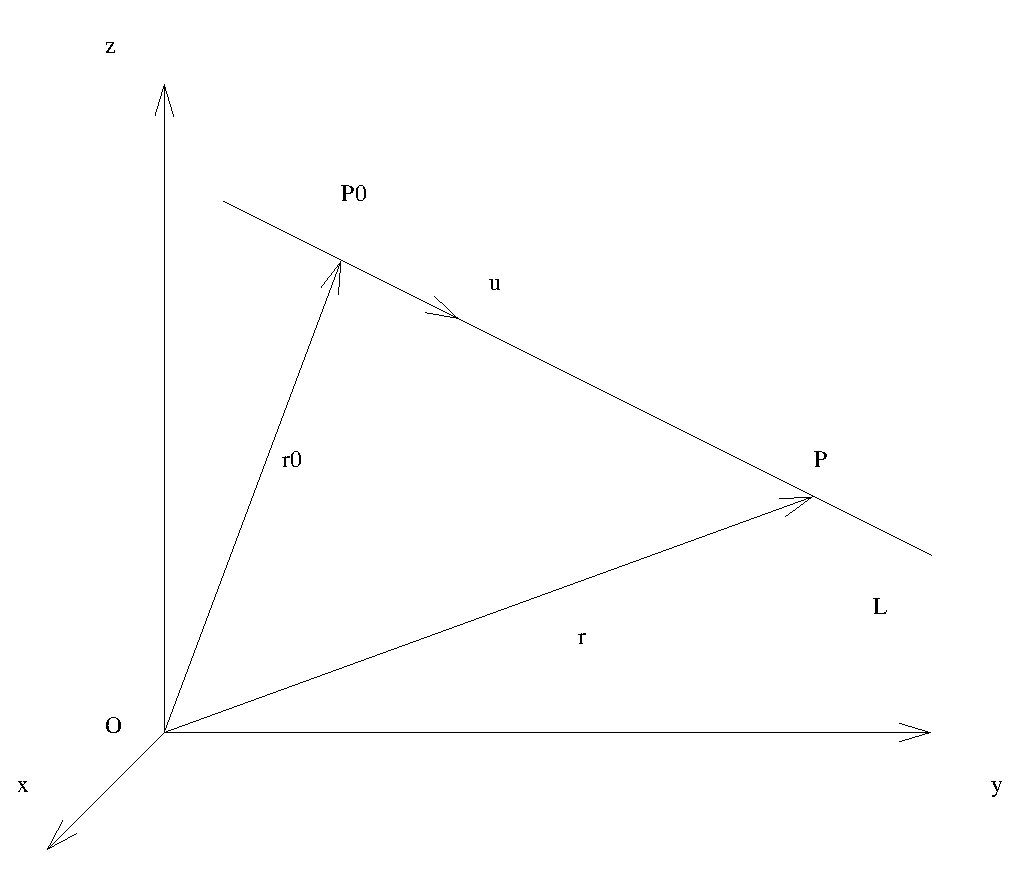
\includegraphics[height=2in]{../../modules/vectors/pictures/ok-line_point_direction_scalar.eps}
    \end{figure}
\end{columns}
\end{frame}

\begin{frame}
\uncover<1->{ $$\left\{ \begin{array}{ll}
           x & = x_0 + t u_1 \\
	   y & = y_0 + t u_2 \\
           z & = z_0 + t u_3
          \end{array}
\right. \Longrightarrow \boxed{\frac{x-x_0}{u_1} = \frac{y-y_0}{u_2} = \frac{z-z_0}{u_3}} \text{ \textcolor[rgb]{0.98,0.00,0.00}{Symmetric equations}}$$}

\uncover<2->{Caution! If $u_2=0$ (for example), then:
%
$$\frac{x-x_0}{u_1} = \frac{z-z_0}{u_3} \quad  \text{ and } \quad y=y_0 $$}

\uncover<3->{Example: Line with direction $\textbf{u} = \langle 4,5,6\rangle$ through $P_0(1,2,3)$:}
\begin{itemize}
 \item<4-> Parametric vectorial equation:
%
$$\textbf{r} = \langle 1,2,3\rangle + t \langle 4,5,6\rangle \leftrightarrow
\textbf{r} = \langle 1+4t, 2+5t, 3+6t\rangle$$
%
\item<5-> Parametric scalar equations:
%
$$\left\{ \begin{array}{ll}
           x & = 1 + 4t \\
	   y & = 2+5t \\
           z & = 3+6t
          \end{array}
\right. , \quad t \text{ real number.}$$
%
\item<6-> Symmetric equations:
%
$$\frac{x-1}{4} = \frac{y-2}{5} = \frac{z-3}{6}\; .$$
\end{itemize}

\end{frame}
\end{problem}

\subsubsection{Line from two points}
\begin{problem}
\begin{frame}
 \frametitle{Line from Two Points}

\begin{columns}

\column{0.4\textwidth}
\psset{xunit=1.4cm, yunit=1.4cm}
\begin{pspicture}(-1,-0.4)(2,2.1)
\fcBoundingBox{-0.8}{-0.4}{4}{2.1}
\renewcommand{\fcScreen}{[-3 -1 -0.2] 0}
\tiny
\uncover<5->{\fcAxesIIId{2}{2}{2}}
\fcLineIIId{[0.5 0.5 1]}{[3 3 0.5]}
\fcLineIIId{[0.5 0.5 1]}{[4 4 0.3]}
\fcLineIIId[arrows=->]{[0 0 0]}{[1 1 0.9]}
\fcPutIIId[br]{[0.5 0.5 0.45]}{$\fcv r_0~$}

\fcLineIIId[linecolor=blue, arrows=->]{[1 1 0.9]}{[2.5 2.5 0.6]}
\fcPutIIId[br]{[1.75 1.75 0.8]}{$\fcv u$}

\fcLineIIId[arrows=->]{[0 0 0]}{[2.5 2.5 0.6]}
\fcPutIIId[b]{[1.25 1.25 0.3]}{$\fcv r_1$}

\fcDotIIId{[1 1 0.9]}
\fcPutIIId[lb]{[1 1 0.95]}{$P_0\uncover<5->{(x_0,y_0, z_0)} $}
\fcDotIIId{[2.5 2.5 0.6]}
\fcPutIIId[lb]{[2.5 2.5 0.65]}{$P_1\uncover<5->{(x_1, y_1, z_1)}$}
\fcDotIIId{[3.5 3.5 0.4]}
\fcLineIIId[arrows=->]{[0 0 0]}{[3.5 3.5 0.4]}
\fcPutIIId[b]{[1.75 1.75 0.2]}{$\fcv r$}
\fcPutIIId[b]{[3.5 3.5 0.5]}{$~P(x,y,z)$}
\fcPutIIId[t]{[4 4 0.3]}{$~L$}
\fcPutIIId[r]{[0 0 0.1]}{$O~~$}
\end{pspicture}
\column{0.6\textwidth}
\begin{itemize}
\item Given: distinct points $P_0$ and $P_1$, position vectors $\textbf{r}_0$ and $\textbf{r}_1$.
\item Goal: write equations of line $L$ through $P_0$ and $P_1$.
\item<2-> Direction of $L$: $\textbf{u} = \textbf{r}_1 - \textbf{r}_0$.
\item<5-> $\fcv{u} = \langle x_1-x_0,y_1-y_0,z_1-z_0\rangle$
\end{itemize}. 
\end{columns}
\uncover<3->{
\begin{definition}
\alert<1->{Parametric vectorial equation} of a line $L$:\\
$
\textbf{r} = \textbf{r}_0 + t(\textbf{r}_1-\textbf{r}_0)
\quad \Leftrightarrow \quad   \textbf{r} = (1-t)\textbf{r}_0 + t\textbf{r}_1
$

\uncover<5->{
\alert<1->{Parametric scalar equations} of a line $L$:
$\left|
\begin{array}{ll}
x & = x_0 + t(x_1-x_0) \\
y & = y_0 + t(y_1-y_0) \\
z & = z_0 + t(z_1-z_0)
\end{array}
\right. \Leftrightarrow \left| \begin{array}{ll}
x & = (1-t)x_0 + tx_1 \\
y & = (1-t)y_0 + ty_1 \\
z & = (1-t)z_0 + tz_1
\end{array}
\right. , \quad t \text{ real number.}$
} %uncover
\end{definition}
} %uncover
\end{frame}
\end{problem}

\begin{problem}
\label{problemEquationsAllDiagonalsCubeContainingOrigin}
We recall that the 8 points $(1,1,1), (-1,1,1), (1,-1,1), (-1,-1,1), (1,1,-1)$, $(-1,1,-1), (1,-1,-1), (-1,-1,-1)$ (all possible sign combinations) give the vertices of a cube with edge 2 units.
 
Find equations for all lines connecting two vertices in the cube above that pass through the origin (how many connecting two vertices of a cube are there? How many of them are edges?).


\answer{ There are $4$ such edges. See the solution below for their equations.
}
\end{problem}
\solution{\ref{problemEquationsAllDiagonalsCubeContainingOrigin}.
A cube has a total of $8 $ vertices. A line is given by two (distinct) points, therefore there are $\binom {8}{2}= \frac{8\cdot 7}{2}= 28$ total lines connecting two distinct vertices of a cube. Of those $12$ lines are cube edges, $12 = 6\cdot 2$ are diagonals of cube faces, and $4 $ are inner diagonals. All four inner diagonals contain the origin. A justification for this can undoubtedly be given by writing all $28$ line equations. However, the origin is in the center of the cube, and we know from our every-day geometric intuition that only the inner diagonals contain the center of a cube; we give no further justification.

The $4$ inner diagonals of the cube, call them $L_1, L_2, L_3, L_4$ pass through the points 

$\begin{array}{rcl}
(1,1,1), (-1,-1,-1) &\in& L_1\\
(1,1,-1), (-1,-1,1) &\in& L_2\\
(1,-1,1), (-1,1,-1) &\in& L_3\\
(-1,1,1), (1,-1,-1) &\in& L_4
\end{array}.
$

Therefore equations for these lines are given by:
$
\begin{array}{rl}
L_1:&  t\langle 1, 1, 1 \rangle\\
L_2:&  t\langle 1, 1, -1 \rangle\\
L_3:&  t\langle 1, -1, 1 \rangle\\
L_3:&  t\langle -1, 1, 1 \rangle\\
\end{array}
$.
}

\subsection{Planes}
\subsubsection{Plane from point and normal}
\begin{problem}
Find an equation of the plane passing through the given point and with the given normal. Find parametric vectorial equations of the plane.

\begin{enumerate}
\item $P_0(2,3,5) $,  $\fcv n= \langle-3, -5, -7 \rangle$.
\item $P_0(1, 1, 1)$, $\fcv n= \langle 1,1,1 \rangle$.
\end{enumerate}
\end{problem}
\solution{\ref{problemFindPlaneFromP(1,2,3)andn(4,5,6)}
As studied, an equation passing through $(1,2,3)$ and with normal $(4,5,6)$ has equation:

\[
\begin{array}{rcl}
\langle x, y, z\rangle\cdot \langle 4,5,6\rangle&=& \langle4,5,6\rangle\cdot \langle 1,2,3\rangle\\
4x +5y+6z&=&23
\end{array}
\]
To find parametric equations of the plane, we need to find two directions, $\fcv u, \fcv v$, that can be added to the base point to obtain all points in the plane. This means that a direction vector $\fcv u$ has to be perpendicular to $\fcv n$. Equivalently, a direction vector $\fcv u$ lies in the plane passing through the origin and orthogonal to $\fcv n$. This means $\fcv u\langle u_1, u_2, u_3\rangle$ satisfies the equation:
\begin{equation}\label{eqproblemFindPlaneFromP(1,2,3)andn(4,5,6)eq1}
\begin{array}{rcl}
\fcv u\cdot \fcv n&=&0\\
4 u_1+5u_2+6u_3&=&0.
\end{array}
\end{equation}
There are infinitely many solutions to that equation - in fact, for each point in the plane passing through the origin and orthogonal to $\fcv n$ there is one solution. However, we only need to find two such non-colinear solutions, and declare them to be our vectors $\fcv u$ and $\fcv v$. It is very easy to do that: if we set $u_1$ and $u_2$ to be arbitrary, then $u_3$ can always be chosen so as to make the equation above hold. There are a number of accepted ways to choose $u_1$ and $u_2$ in a not-so-arbitrary fashion. For reasons outside of the scope of this homework, such ways to choose $u_1$ and $u_2$ may be preferable to the choosing at random. Our scheme for choosing a vector $\fcv u$ will be to choose $u_1=1$ and $u_2=0$ (or the other way round for $\fcv v$), and then to rescale the resulting vector so all coordinates are integers and the first non-zero coordinate is positive. In other words, we select $\fcv u$ to be proportional to $\langle 1, 0, -\frac{4}{6} \rangle$, and $\fcv v$ to be proportional to $\langle 0, 1 ,-\frac{5}{6} \rangle$, i.e., we select
\[
\begin{array}{rcl}
\fcv u&=& \langle 3,0, -2 \rangle \\
\fcv v&=& \langle 0, 6, -5 \rangle
\end{array}. 
\] 
Finally we get that a parametric equation of the plane is given by:
\begin{equation}\label{eqproblemFindPlaneFromP(1,2,3)andn(4,5,6)eq2}
\langle 1,2,3 \rangle + s\langle 3,0, -2 \rangle +t\langle 0, 6, -5 \rangle\quad .
\end{equation}
The above equations are not unique; therefore our problem has many correct answers. 

A question arises: what do we need to do in order to check if two plane parametrizations are equivalent? Equivalently, how do we check that equation \eqref{eqproblemFindPlaneFromP(1,2,3)andn(4,5,6)eq2} gives a plane that coincides with the plane in given in \eqref{eqproblemFindPlaneFromP(1,2,3)andn(4,5,6)eq1}? Here's what we need to do to make sure our answer is correct (we leave the justification for that to the reader):
\begin{itemize}
\item Check that our $\fcv u, \fcv v$ are orthogonal to $\fcv n$. 
\item Check that our $\fcv u, \fcv v$ are not proportional to one another. 
\item Check that the base point of our equation is in the original plane. 
\end{itemize}

}

\subsubsection{Plane from point and two directions}
\begin{problem}
Find an equation of plane $\mathcal P$ passing through the point and parallel to the given directions.

\begin{enumerate}
\item $P_0(1,2,3)$, $\fcv u=(2,3,5)$, $\fcv v=(3,5,7 )$.

\answer{$\mathcal P: z+y-4 x-1 =0$}
\item $P_0(1,1,1)$, $\fcv u=(1,-1,0)$, $\fcv v= (0,1,-1)$.
\answer{$\mathcal P:  z+y+x-3  =0$}
\end{enumerate}

\end{problem}

\subsubsection{Plane from three points}
\begin{problem}
\begin{frame}
 \frametitle{Plane from Three Points}

\begin{columns}
\column{0.4\textwidth}
\psset{xunit=0.8cm, yunit=0.8cm}
\begin{pspicture}(-0.2, -0.2)(3,3)
\tiny
\renewcommand{\fcScreen}{[-2 -1 -0.5] 0}
\fcParallelogramIIId{[-0.8 -0.8 3.6]}{[-1.4 2.4 1]}{[2.4 -1.4 1]}
\fcPutIIId[l]{[0 0 0.05]}{$~~O$}
\fcDotIIId{[0 0 0]}

\fcLineIIId[arrows=->, linestyle=dotted]{[0 0 0]}{[2 0 0]}
%\fcPutIIId{[1 0 0]}{$\fcv r_2$}
\fcLineIIId[arrows=->, linestyle=dotted]{[0 0 0]}{[0 2 0]}
%\fcPutIIId{[0 1 0]}{$\fcv r_0$}
\fcLineIIId[arrows=->, linestyle=dotted]{[0 0 0]}{[0 -0.4 2.4]}
%\fcPutIIId{[0 -0.2 1.2]}{$\fcv r_1$}
\fcDotIIId{[2 0 0]}
\fcDotIIId{[0 2 0]}
\fcDotIIId{[0 -0.4 2.4]}
\fcPutIIId[r]{[2 0 0]}{ $P_2(\fcv r_2)~$}
\fcPutIIId[tl]{[0 2 0]}{ $P_0(\fcv r_0)$}
\fcPutIIId[b]{[0 -0.4 2.4]}{ $P_1(\fcv r_1)$}
\fcLineIIId[arrows=->]{[0 2 0]}{[2 0 0]}
\fcPutIIId[t]{[1 1 -0.1]}{$~\fcv v$}
\fcLineIIId[arrows=->]{[0 2 0]}{[0 -0.4 2.4]}
\fcPutIIId[b]{[0 0.8 1.3]}{$~\fcv u$}%
\fcPerpendicularIIId{[4.8 6.8 4.8]}{ [0 2 0] [2 0 0]}{0.6}%
\fcPerpendicularIIId[arrows=<-]{[4.8 6.8 4.8]}{[0 2 0] [0 -0.4 2.4]}{0.6}%
\fcLineIIId[linestyle=dotted]{[0 0 0]}{[1.4 -0.84 1.44]}%
\fcPerpendicularIIId[arrows=<-]{[4.8 6.8 4.8]}{[0 2 0] [1.4 -0.84 1.44]}{0.8}%
\fcLineIIId[arrows=->]{[0 2 0]}{[1.4 -0.84 1.44]}%
\fcPutIIId[b]{[1.4 -0.84 1.44]}{$P(\fcv r)$}%
\end{pspicture}

\column{0.6\textwidth}
\begin{itemize}
\item Given: three non-collinear points $P_0(\fcv{r}_0)$, $P_1(\fcv{r}_1)$, $P_2(\fcv{r}_2)$.
\item Goal: find equations fo plane $\mathcal{P}$ passing through $P_0$, $P_1$, and $P_2$.
\item<2-> The plane is parallel to $\fcv{u} = \fcv{P}_0\fcv{P}_1 = \fcv{r}_1 -\fcv{r}_0$ and passing through $P_0$ $\Rightarrow$ this problem was solved previously.

\end{itemize}
\end{columns}
\only<3>{
Normal $\fcv{n} = \fcv{u} \times \fcv{v} =
(\fcv{r}_1-\fcv{r}_0) \times (\fcv{r}_2-\fcv{r}_0)$  \\

\alert<1->{Implicit equation}:
$$(\fcv{r}-\fcv{r}_0) \cdot \fcv{n} = 0$$
$$\boxed{(\fcv{r}-\fcv{r}_0) \cdot [(\fcv{r}_1-\fcv{r}_0) \times (\fcv{r}_2-\fcv{r}_0)] = 0}$$
$$\text{Vol}(R(\fcv{P}_0\fcv{P}, \fcv{P}_0\fcv{P}_1, \fcv{P}_0\fcv{P}_2)) = 0$$
}

\only<4>{
\alert<1->{Implicit equation}: $(\fcv{r}-\fcv{r}_0) \cdot [(\fcv{r}_1-\fcv{r}_0) \times (\fcv{r}_2-\fcv{r}_0)] = 0$

Let the points have coordinates $P_0(x_0,y_0,z_0)$, $P_1(x_1,y_1,z_1)$, $P_2(x_2,y_2,z_2)$. $P(x,y,z)$ is on plane $\mathcal{P}$:

\alert<1->{Implicit scalar equation}:
$\left| \begin{array}{ccc}
x-x_0 & y-y_0 & z-z_0 \\
x_1-x_0 & y_1-y_0 & z_1-z_0 \\
x_2-x_0 & y_2-y_0 & z_2-z_0
\end{array}
\right| = 0\; .$
}

\vskip 10cm
\end{frame}


\end{problem}

\subsection{Distances between points, lines, planes}
\subsubsection{Distance between line and point}
\begin{problem}
Find the distance between the line and the point.

\begin{enumerate}
\item The line passing through $P_0(1,1,1)$ and $P_1(-1,-1,-1)$ and the point $Q(1,0,0)$.
\answer{$\frac{\sqrt{6}}{3} $}
\item The line passing through $P_0(-2,3,-5)$ and $P_1(3,4,5)$ and the point $Q(2,-2,2)$. 
\answer{$\frac{\sqrt{57610}}{42}$}
\end{enumerate}


\end{problem}
\subsubsection{Distance between plane and point}
\begin{problem}
Find the distance between the plane and the point.

\begin{enumerate}
\item The plane passing through $P_0(1,2,3) $, $P_1(2,3,5)$ and $P_2(3,5,7)$ and the point $Q(2,-2,2)$.
\answer{$\frac{3}{5}\sqrt{5}$}
\item The plane passing through $P_0(1,2,3) $, $P_1(2,3,5)$ and $P_2(3,5,7)$ and the point $Q(5,7,11)$.
\answer{$0$}
\item The plane passing through the points $P_0(1,1,1)$, $P_1(1,-1,-1)$, $P_2(-1,-1,1)$ and the point $Q(-1,1,-1)$.
\answer{$\frac{4}{3}\sqrt{3}$}
\end{enumerate}

\begin{comment}
Calculator code to solve above problem:

p0:=(1,2,3); 
p1:=(2,3,5);
p2:=(3,5,7);
q:=(2,-2,2);
u1:=p1-p0;
u2:=p2-p0;
u:=q-p0;
n:=u1\times u2;
((u n^t)_1)_1 /\sqrt{}(((n n^t)_1)_1) 
\end{comment}
\end{problem}

\subsubsection{Distance between lines}
\begin{problem}
Recall that a regular tetrahedron can be realized using 4 vertices of a cube. 

Find the distance between two opposite edges of a regular tetrahedron inscribed in a 2x2x2 cm cube.
\end{problem}
\begin{problem}
\begin{frame}
\frametitle{Distance between non-parallel lines}
\begin{columns}
\column{0.4\textwidth}
\begin{pspicture}(-2, -2)(2,2)
\tiny
\renewcommand{\fcScreen}{[-1 0 -0.5] 0}
\fcBoundingBox{-2}{-2}{2}{2}
\uncover<2->{%
\fcParallelogramIIId{[1.2 -1.2 1]}{[1.2 1.2 1]}{[-1.2 -1.2 1]}
\fcPutIIId[b]{[-1.2 -1.2 1]}{$\mathcal P$}
}%
\fcLineIIId{[-1 -1 -1]}{[1 1 -1]}
\fcLineIIId{[1 -1 1]}{[-1 1 1]} 
%\fcPerpendicularIIId[arrows=->, linecolor=green]{[0 0 -1]}{[1 -1 1] [-1 1 1]}{0.2}
\fcPutIIId[l]{[-1 1 1]}{$~~L_1$}
\fcPutIIId[r]{[-1 -1 -1.2]}{$L_2$}
\uncover<6->{%
\fcLineIIId[linestyle=dotted]{[0 0 1.3]}{[0 0 -1.3]}%
\fcPutIIId[rt]{[-0.1 0.1 -1]}{$Q_2~~~$}%
}%
\uncover<10->{%
\fcPerpendicularIIId[linestyle=none]{[0 0 -0.125]}{[0 0 1] [1 1 1]}{0.2}%
\fcPerpendicularIIId[linestyle=none]{[0 0 -0.125]}{[0 0 1] [-1 1 1]}{0.2}%
}%
\uncover<13->{%
\fcLineIIId[arrows=->, linecolor=green]{[0.8 -0.8 1]}{[0.9 0.9 -1]}%
\fcLineIIId[arrows=->, linecolor=green]{[0 0 1]}{[0.1 1.7 -1]}%
\fcDotIIId{[0.1 1.7 -1]}%
\fcPutIIId[l]{[0.1 1.7 -1]}{$~~R$}%
\fcPutIIId[l]{[0.05 0.85 0]}{$\fcv r_2- \fcv r_1$}%
}%
\uncover<6->{%
\fcPerpendicularIIId{[0.8 0.8 -1]}{[0 0 -1]}{0.2}
}%
\uncover<14->{\fcLineIIId[arrows=->, linecolor=brown]{[0.8 -0.8 1]}{[0 0 1]}%
\fcLineIIId[arrows=->, linecolor=brown]{[0.9 0.9 -1]}{[0.1 1.7 -1]}%
}%
\uncover<15->{%
\fcPerpendicularIIId{[0.1 1.7 -1]}{[0 0 -1]}{0.2}%
}%
\uncover<11->{%
\fcLineIIId[arrows=->, linecolor=blue]{[0 0 1]}{[0 0 -0.125]}%
\fcPutIIId[r]{[0 0 0.4375]}{$\fcv n~$}
}%
\uncover<4->{%
\fcLineIIId[linestyle=dotted]{[-1 -1 1]}{[1 1 1]}
\fcPutIIId[l]{[1 1 1]}{$~~L_2'$}
}%
\fcLineIIId[linecolor=red, arrows=->]{[0 0 -1]}{[0.75 0.75 -1]}
\fcPutIIId[t]{[0.325 0.325 -1.1]}{$\fcv u_2$}
\fcDotIIId{[0 0 -1]}
\uncover<12->{%
\fcDotIIId{[0.8 -0.8 1]}%
\fcPutIIId[br]{[0.8 -0.8 1]}{$P_1~$}%
\fcDotIIId{[0.9 0.9 -1]}%
\fcPutIIId[tr]{[0.9 0.9 -1]}{$P_2~$}%
}%
\uncover<5->{%
\fcDotIIId{[0 0 1]}
\fcPutIIId[r]{[-0.1 0.1 1]}{$Q_1~~~$}
}%
\fcLineIIId[linecolor=red, arrows=->]{[0 0 1]}{[-0.75 0.75 1]}
\fcPutIIId[br]{[-0.325 0.325 1]}{$\fcv u_1$}
\uncover<2->{
\fcLineIIId[linecolor=red, arrows=->]{[0 0 1]}{[0.75 0.75 1]}
\fcPutIIId[t]{[0.325 0.325 0.9]}{$\fcv u_2$}
}
%\fcPutIIId{[2 2 0]}{%
%\fcLineIIId[linecolor=red, arrows=->]{[0 0 1]}{[-0.75 0.75 1]}
%\fcPutIIId[br]{[-0.325 0.325 1]}{$\fcv u_1$}
%\fcLineIIId[linecolor=red, arrows=->]{[0 0 1]}{[0.75 0.75 1]}
%\fcPutIIId[t]{[0.325 0.325 0.9]}{$\fcv u_2$}
%}%
\end{pspicture}

\column{0.6\textwidth}
\begin{itemize}
\item Given: lines $\begin{array}{rrcl}L_1: & \fcv{r}&=& \fcv{r}_1+t\fcv{u}_1 \\ L_2:& \fcv{r} &=& \fcv{r}_2+s\fcv{u}_2\end{array}$
\item The lines are skew or intersecting, i.e., $\fcv{n} = \fcv{u}_1 \times \fcv{u}_2 \neq \fcv{0}$.
\item Goal: find distance between the lines = $d(L_1, L_2)$ = shortest distance b-n points on the two lines.
\end{itemize}
\end{columns}
\begin{itemize} 
\only<handout:1|1-8>{
\item<2-> Construct plane $\mathcal P$ with directions $\fcv u_1$, $\fcv u_2$ and passing through $L_1$. 
\item<3-> Distance b-n $L_2$ and points on $\mathcal P$ is constant.
\item<4-> Project $L_2$ orthogonally on $\mathcal P$; let the projection be $L_2'$.
\item<5-> Let $L_2' $ and $L_1$ intersect in point $Q_1$.
\item<6-> Let $Q_2$ be the heel of the perpendicular from $Q_1$ onto $Q_2$.
\item<7-> $\Rightarrow$ $Q_1Q_2=d(L_1, L_2)$.
}
\only<handout:1|8-16>{
\item \alert<8,9>{$|Q_1Q_2|=d(L_1, L_2)$}.
}
\only<handout:2|9-16>{
\item<10-> $\fcv Q_1\fcv Q_2 \perp L_1, L_2$ \uncover<11->{$\Rightarrow$  $\fcv Q_1 \fcv Q_2$ is proportional to $\fcv n = \fcv u_1\times \fcv u_2$.}
\item<12-> Pick arbitrary points on $L_1, L_2$ - say, the base points $P_1(\fcv r_1), P_2(\fcv r_2)$.
\item<13-> Let $R$ be such that $\fcv Q_1\fcv R=\fcv P_1 \fcv P_2=\fcv r_2-\fcv r_1$. 
\item<14-> Then $\fcv{P}_2\fcv R$ is proportional to $\fcv u_1$.
\item<15-> $\Rightarrow $ $\fcv Q_2\fcv R= \fcv Q_2  \fcv P_2+\fcv{P}_2\fcv{R}$ is perpendicular to $\fcv n$.
}
\only<handout:3|16->{
\item<16->\alert<16,17>{ $\Rightarrow$ $\fcv Q_1 \fcv Q_2= \fcv {proj} _{\fcv n} (\fcv r_2-\fcv r_1)$.}
}
\only<handout:3|17->{
\item<18-> 
$d(L_1,L_2)  = |\fcv{proj}_{\alert<19>{\fcv{n}}} (\fcv{r}_2-\fcv{r}_1)| \uncover<19->{= \boxed{\frac{|(\fcv{r}_2-\fcv{r}_1)\cdot \alert<19,20>{\fcv{n}} | }{ |\alert<19,20>{\fcv{n}}|}}} \uncover<20->{= \frac{ |(\fcv{r}_2 -\fcv{r}_1 )\cdot (\alert<20>{ \fcv{u}_1\times \fcv{u}_2})|}{ | \alert<20>{\fcv{u}_1\times \fcv{u}_2}|}}$
\item<21-> If lines are intersecting we know $d(L_1,L_2)=0$. \uncover<22->{Since the lines intersect $L_2$ and $L_2'$ coincide.} \uncover<23->{$\Rightarrow$ $(\fcv{r}_2-\fcv{r}_1) \cdot (\fcv{u}_1\times \fcv{u}_2) = 0$} \uncover<24->{$\Rightarrow $ the formula $d(L_1, L_2)= \frac{|(\fcv{r}_2 - \fcv{r}_1 )\cdot (\fcv{u}_1\times \fcv{u}_2)|}{ | \fcv{u}_1\times \fcv{u}_2|}=0$ produces the expected result.}
}
\end{itemize}

\vskip 5cm
\end{frame}


\end{problem}
\solution{\ref{problemDistanceLineLine(1,2,3)(6,5,4)to(1,3,5)(2,4,6)}
We need to first establish whether the two lines are parallel. Let $\fcv u$ be the direction vector of the first line given by
\[\fcv u=\fcv Q_0 \fcv Q_1= ( 6,5,4)-( 1,2,3) = (5,3,1)
\]
and let $\fcv v$ be the direction vector of the second line given by
\[
\fcv v=\fcv P_0 \fcv P_1= (2,4,6 )-(1,3,5)=( 1, 1, 1).
\]
Now it is straightforward to see that the two lines are not parallel - indeed, one immediately sees that $\fcv u= (5,3,1)$ is not a scalar multiple of $\fcv v=(1,1,1)$. Since the two lines are not parallel, the two direction vectors determine a plane through the origin whose normal vector is given by
\[
\fcv n= \fcv u\times \fcv v=  (5,3,1)\times ( 1, 1, 1)= \left| \begin{array}{ccc} \fcv i & \fcv j &\fcv k\\ 5&3&1 \\1 &1 &1\end{array}\right|= 2\fcv i -4\fcv j+ 2\fcv k= (2, -4, 2)\quad .
\]
We note that if the vectors $\fcv u, \fcv v$ were parallel, then the cross product above would had been zero. Now the distance between the two lines is obtained by taking an arbitrary vector with tail on one line and head on the other, and computing the length of its projection it onto $\fcv n $. We use the vector $\fcv r= \fcv Q_0\fcv P_0$. Then the distance $d$ between the two lines is given by:
\[
d=\frac{|\fcv r \cdot \fcv n| }{|\fcv n|}= \frac{|\left(( 1,3,5) - ( 1,2,3)\right) \cdot \fcv  n|}{|\fcv n|}=\frac{ |( 0, 1, 2 )\cdot( 2, -4,2 )|}{|\fcv n|}=0.
\]
Therefore the distance between the two lines is zero. This completes our solution.

We note that since the distance between the lines is zero, they must intersect. As a consistency check for our work, let us verify that the two lines do indeed intersect. The first line is parametrized by $( 1,2,3)+t( 5,3,1) $ i.e., has parametric equations

\[
\left|\begin{array}{rcl}x&=& 1 +5t \\y&=&2+3t\\z&=&3+t \end{array}\right.\quad .
\]
Similarly, the second line is given by the equations
\[
\left|\begin{array}{rcl}x&=& 1 +s \\y&=&3+s\\z&=&5+s \end{array}\right.\quad .
\]
Therefore to find an intersection of the two lines, we need to solve the system
\[
\left|\begin{array}{rcl} 1 +5t&=&1+s \\2+3t&=&3+s\\3+t&=&5+s \end{array}\right.\quad.
\]
From the first equality we get that $s=5t$. We substitute that into the second equality to get that $t=-\frac{1}{2}$. Therefore the intersection of the two lines is the point

\[
(1,2,3)-\frac{1}{2}(5,3,1)= \left(-\frac{3}{2}, \frac{1}{2}, \frac{5}2\right)= (1,3,5)-\frac{5}{2}(1,1,1)\quad ;
\]
all our error checks have been successful.
}

\solution{\ref{problemDistanceLineLine(1,3,4)(2,3,1)to(1,2,2)(0,2,5)}
We present a solution in a concise form suitable for exam taking.

Let $L_1, L_2$ be the two lines.
\[
\begin{array}{rcll|l}
\fcv u &=& (2,3,1)-(1,3,4)=(1,0,-3)&& \text{direction vector } L_1\\
\fcv v &=& (0,2,5)-(1,2,2)=(-1,0,3)=-\fcv u&&\text{direction vector } L_2\\
&&\text{Therefore } L_1 \parallel  L_2\\
\fcv r&=&(2,3,1)-(0,2,5)=(2,1,-4) &&\text{arbitrary vector connecting } L_1, L_2\\
L_1\parallel L_2\Rightarrow\\
\text{dist}(L_1,L_2)&=&|\fcv{orth}_{\fcv u} \fcv r| \\
&=&\left|\fcv r- \fcv {proj}_{\fcv u} \fcv r \right|\\
&=&\left|\fcv r- \frac{\fcv r \cdot \fcv u}{|\fcv u|^2}\fcv{u} \right|\\
&=&\left| (2,1,-4)-\frac{(2,1,-4)\cdot (1,0,-3)}{1^2+0^2+(-3)^2}(1,0,-3) \right|\\
&=&\left|\left(\frac{3}{5}, 1, \frac{1}{5} \right)\right|\\
&=&\sqrt{\left(\frac{3}{5}\right)^2+ 1^2+ \left(\frac{1}{5}\right)^2 }\\
&=&\frac{\sqrt{35}}{5} \quad .
\end{array}
\]
}

\solution{\ref{problemDistanceLineLine(1,3,4)(2,3,1)to(1,2,2)(0,2,4)}
We present a solution in a concise form suitable for exam taking.
\[\begin{array}{rcll|l}
\fcv u &=& (2,3,1)-(1,3,4)=(1,0,-3)&& \text{direction vector } L_1\\
\fcv v &=& (0,2,4)-(1,2,2)=(-1,0,2)=-\fcv u&&\text{direction vector } L_2\\
\fcv r &=& (1,3,4)-(1,2,2)=(0, 1, 2)  &&\text{arbitrary vector connecting } L_1,L_2\\
\fcv n&=&u\times v=(0, 1, 0) &&\neq 0\Rightarrow L_1\not \parallel L_2\\
L_1\not \parallel L_2\Rightarrow \\
\text{dist}(L_1,L_2)&=&\left|\fcv {proj}_{\fcv n} \fcv r\right|\\
&=&\left|\fcv r \cdot \frac{\fcv n}{|\fcv n|}\right|\\
&=&\left| (0,1,2)\cdot (0,1,0)\right|\\
&=&1\quad .
\end{array}
\]
}


\subsection{Angles (in space)}
\subsubsection{Angles between lines}
\begin{problem}
Recall that a regular tetrahedron can be realized using 4 vertices of a cube. 

Find the angle between two edges of a regular tetrahedron. 
\end{problem}

\subsubsection{Angle between plane and line}
\begin{problem}
Find the angle between the line and the plane.

\begin{itemize}
\item The line passing through $(-1,-1,-1) $ and $(1 , 1, 1)$ and the plane with equation $z=-1$.
\item The line passing through $(2,3, 5)$ and $(3,5,7)$ and the plane passing through $(1,0,0)$, $(0,1,0)$ and $(0,0,1)$.
\end{itemize}
\end{problem}

\begin{problem}
Recall that a regular tetrahedron can be realized using 4 vertices of a cube. Find the angle between an edge of a regular tetrahedron and one of the two sides of the tetrahedron not containing the edge.
\end{problem}

\subsubsection{Angles between planes}
\begin{problem}
Recall that a regular tetrahedron can be realized using 4 vertices of a cube.

Find the angle between two faces of a regular tetrahedron.
\end{problem}

\section{Polar, Cylindrical and Spherical coordinates}
\subsection{Polar coordinates}
\begin{problem}
Find polar equations of the line given below.

\begin{enumerate}[ref={\fcProblemRef}]
\item The line $x+y=1$.
\answer{$\begin{array}{rcl} r(\cos \theta +\sin \theta)&=&1 \\ r=\frac{\sqrt{2}}{2}\sec \left(\theta -\frac{\pi}{4}\right) \end{array} $}
\item \label{problemWriteInPolarx+sqrt(3)y=2} The line $ x+\sqrt{3}y=2$.
\answer{ $\begin{array}{rcl} r\left(\frac{1}{2}\cos \theta +\frac{\sqrt{3}}{2}\sin \theta\right)&=& 1 \\ r=\sec \left(\theta-\frac{\pi}{3} \right) \end{array}$}
\item The line passing through $(3,5)$ and $(5,7)$.

\answer{$\begin{array}{rcl} x-y&=&-2\\ r(\cos \theta -\sin \theta)&=&-2\\ r=-\sqrt{2}\sec\left(\theta+\frac{\pi}{4} \right) \end{array} $}
\item The line passing through $(2,3)$ and $(-3,-2)$.
\answer{$\begin{array}{rcl} x-y&=&-1\\ r(\cos \theta -\sin \theta)&=&-1\\ r=-\frac{\sqrt{2}}{2} \sec \left( \theta + \frac{ \pi }{4} \right) \end{array} $}
\end{enumerate}
\end{problem}

\solution{\ref{problemWriteInPolarx+sqrt(3)y=2}

Polar coordinates are given by
\[
\left|\begin{array}{rcl}
x&=& r\cos \theta\\
y&=& r\sin \theta 
\end{array}\right. .
\]
All we need to do to obtain polar equations for our line is substitute the above expressions in the equation for the line. 
\[
r\cos \theta + \sqrt{3}r\sin \theta= 2.
\]
This is a perfectly good answer, but we can transform the equation to make it look more compact:
\[
\begin{array}{rcll|l}
\displaystyle r\cos \theta + \sqrt{3}r\sin \theta&=&\displaystyle 2\\
\displaystyle r\underbrace{\frac{1}{2}}_{=\cos \left(\frac{\pi}{3}\right)} \cos\theta +r \underbrace{\frac{\sqrt{3}}{2}}_{=\sin \left(\frac{\pi}{3}\right)} \sin\theta &=&\displaystyle  1 \\
\displaystyle r\cos \left(- \frac{\pi }{3}\right)\cos \theta -\sin \left(- \frac{\pi }{3}\right)\sin \theta &=& 1&&   \text{use } \cos (a+b)= \cos a \cos b - \sin a \sin b\\
\displaystyle r\cos (\theta -\frac{\pi}{3})&=&1\\
r&=&\displaystyle \frac{1}{\cos \left(\theta - \frac{\pi}{3} \right)}\\
&=&\displaystyle \sec\left (\theta - \frac{\pi}{3}\right )\quad .

\end{array}
\]


}

\begin{problem}
Find polar equations of the circle given below.

\begin{enumerate}
\item The circle given by $(x-1)^2+y^2=1$.
\answer{$r=2\cos \theta$}
\item The circle given by $x^2+ x+y^2=1$.
\answer{$r^2+r\cos \alpha -1=0$}
\item The circle with center $(1,2)$ and radius $3$.
\answer{$r^{2} -4 r \sin{}\theta-2 r \cos{}\theta-4 =0$}
\item The circle with center $(2,3)$ and radius $4$.
\answer{$r^{2} -6 r \sin{}\theta-4 r \cos{}\theta-3 =0$}
\end{enumerate}
\end{problem}
\subsection{Cylindrical coordinates - basics}

\begin{problem}
Find an equation of the plane in cylindrical coordinates.

\begin{enumerate}
\item The plane given by $x+y+z=1$.
\item The plane given by $2x+3y-5z=0$.
\item The plane passing through $(-1, 1, 1)$, $(1, 1, -1)$ and $(1, -1, 1)$.
\item The plane passing through $(2,3,5 )$, $(3, 5, 2)$ and $(5, 2, 3)$.
\end{enumerate}
\end{problem}

\begin{problem}
Find an equation of the sphere in cylindrical coordinates.

\begin{enumerate}
\item The unit sphere.
\item The sphere with equation $x^2 +x+ y^2+2y + z^2 +3z=0$.
\item The sphere with center $(1,2,3)$ and radius $5$.
\end{enumerate}
\end{problem}
\subsection{Spherical coordinates - basics}

\begin{problem}
Find an equation of the plane in spherical coordinates.

\begin{enumerate}
\item The plane given by $x+y+z=1$.
\item The plane given by $2x+3y-5z=0$.
\item The plane passing through $(-1, 1, 1)$, $(1, 1, -1)$ and $(1, -1, 1)$.
\item The plane passing through $(2,3,5 )$, $(3, 5, 2)$ and $(5, 2, 3)$.
\end{enumerate}
\end{problem}

\begin{problem}
Find an equation of the sphere in spherical coordinates.

\begin{enumerate}
\item The unit sphere.
\item The sphere with equation $x^2 +x+ y^2+2y + z^2 +3z=0$.
\item The sphere with center $(1,2,3)$ and radius $5$.
\end{enumerate}
\end{problem}

\section{Quadratic surfaces}

\begin{problem}
Match the surface graph to its mathematical name and to its equation.

\begin{enumerate}
\item
\begin{pspicture}(-2,-2)
\renewcommand{\fcScreen}{[-2 -1 -0.9] 0}
\fcSurfaceDirectDraw{}{-1}{-1}{1}{1}{[u v u u mul v v mul add]}
\end{pspicture}

\end{enumerate}
\end{problem}

\begin{problem}
Determine the type of the quadratic surface given by the equation.
\begin{enumerate}
\item 
$x^2 +y^2+z^2+x+2y+3z=0$.
\answer{sphere (also ellipsoid)}
\item $x^2 +2y^2+z^2+x+2y+3z=0$.
\answer{(circular) ellipsoid}
\item $x^2 +2y^2+3z^2+x+2y+3z=0$.
\answer{ellipsoid}
\item \label{problemTypeOfSurfacez^2+2y^2-3x^2+x+y+1=0} $z^2+2y^2-3x^2 + x+y+1=0 $.
\answer{(elliptic) hyperboloid one sheet}
\item $z^2-y^2+\frac{1}{4}x^2 + x-y+1=0 $.
\answer{(elliptic) hyperboloid two sheets}
\item $x^2+y^2-\frac{1}{4}z^2 + x-y+5=0 $.
\answer{(circular) hyperboloid one sheet}
\item $\frac{1}{4}x^2-y^2+z^2-x+1=0$
\answer{(elliptic) cone}
\item $-\frac{1}{4}x^2+y^2+z^2-x-1=0$
\answer{(circular) cone}
\item $xy +z^2+1=0$. Hint: write $x=\frac{1}{\sqrt{2}}(u+v)$, $y=\frac{1}{ \sqrt{ 2} } (u-v) $ for some new variables $u,v$. Solve the problem in the $z,u,v$ -coordinates. Argue that the (axes of the) $u,v,z$-coordinate system can be obtained from the $x,y,z$-coordinate system via rotation.
\answer{(circular) hyperboloid one sheet}
\item $x^2+2y^2+z=0 $.
\answer{(elliptic) paraboloid}
\item $x^2+y^2+2xy+z=0 $.
\answer{cylindrical paraboloid}
\item $x^2-y^2+2x+z=0 $.
\answer{parabolic hyperboloid}
\end{enumerate}
\end{problem}
\solution{
\ref{problemTypeOfSurfacez^2+2y^2-3x^2+x+y+1=0}
We have that
\[
\begin{array}{rcl}
\displaystyle z^2+2y^2-3x^2 + x+y+1&=&0\\
\displaystyle z^2+ 2\left(y+\frac{1}{4}\right)^2 - 3\left(x-\frac{1}{6} \right)^2 -\frac{1}{8}+\frac{1}{12}+1&=&0\\
\displaystyle z^2+ 2\left(y+\frac{1}{4}\right)^2 &=&\displaystyle 3\left(x-\frac{1}{6} \right)^2-\frac{23}{24}
\end{array}
\]
This figure is given by sum of two squares equal to a square minus a positive number. That makes is a hyperboloid two sheet, as explained in the theoretical discussions.
\begin{pspicture}(-3, -3)(3,3)
\pstVerb{20 dict begin
/coeffZ 1 def
/coeffY 2 def
/coeffX 3 def
/xFun {v} def
/rightSide {xFun 1 6 div sub dup mul 3 mul 23 24 div sub} def
/xTipTop {23 24 div coeffX div sqrt 1 6 div add} def
/xTipBottom {23 24 div coeffX div sqrt -1 mul 1 6 div add} def
/yFun { u sin 1 4 div sub coeffY sqrt div  rightSide sqrt mul} def
/zFun { u cos coeffZ sqrt div  rightSide sqrt mul} def
}
\renewcommand{\fcScreen}{[-0.3 2 -0.75] -1\space}
\fcStartIIIdScene
\fcAxesIIIdFullInScene{-3}{-3}{-3}{3}{3}{3}
\fcSurfaceInScene[arrows=(none), iterationsV=4, iterationsU=18]{0}{3}{360}{xTipTop 0.004 add}{[xFun yFun zFun]}{}
\fcSurfaceInScene[arrows=(none), iterationsV=4, iterationsU=18]{0}{xTipBottom 0.004 sub}{360}{-3 1 3 div add}{[xFun yFun zFun]}{}
\fcFinishIIIdScene[true]
\fcPutIIId{[3.2 0 0]}{$x$}
\fcPutIIId{[0 3.2 0]}{$y$}
\fcPutIIId{[0 0 3.2]}{$z$}
\pstVerb{end}
\end{pspicture}
}

\section{Curves in space}
\subsection{Curvature}
\begin{problem}
Compute the tangent vector, the normal vector and the curvature at each point on the curve.

\begin{enumerate}[ref={\fcProblemRef}]
\item The equator of the unit sphere $\fcv r(t)= ( \cos t, \sin t ,0 )$.
\item The equator of the unit sphere $\fcv r(t)= ( \cos t, \sin t ,0 )$.
\item The loxodromic curve $\fcv r(t)= ( \cos (10t) \sin (t), \sin (10t)\sin (t), \cos (t) )$. A loxodromic curve is a curve obtained by taking a straight line in the $\{(\rho,\phi, \theta)|\rho =\text{const}\}$-plane in spherical coordinates and mapping it into the $x,y,z$-coordinates. Loxodromic curves were used in navigation: maintaining a course on a loxodromic curve requires only keeping a constant angle with the north direction (which one approximately obtained via compass).

\begin{pspicture}(0,0)(1,1)
\fcCurveIIId[plotpoints=500, linecolor=red]{0}{180}{[10 t mul cos t sin mul 10 t mul sin t sin mul t cos ]}
\end{pspicture}
\item The ellipse $\fcv r(t) = ( a\cos t, b\sin t ) $. Where is the curvature largest? Where smallest? Can you answer without computation, and does your answer match your computation?
\item The loxodromic meridian
$\fcv r(t)=( \sin (at)\cos (bt),  \sin(at)\sin (bt) ,\rho\cos (at) )
$.
\item The trefoil (torus) knot
$\fcv r=( \left( R+r\sin \left(3t\right)\right) \cos (2t) ,(R+r\sin \left( 3t \right) \sin (2t) ,r\cos (3t))
$.
\item The torus curve
$\fcv r=( \left( R+r\sin \left(20t\right)\right) \cos (t) ,(R+r\sin \left( 20t \right) \sin (2t) ,r\cos (20t))
$.

\begin{pspicture}(0,0)(1,1)
\fcAxesIIId{3}{3}{2}

\pstVerb{
6 dict begin
/phi  {t 20 mul} def
/theta {t } def
/R 2 def
/r 0.2 def
/xyRad {phi sin r mul R add} def
/torusCurve {[theta cos xyRad mul theta sin xyRad mul phi cos r mul ]} def
}
\fcCurveIIId[linecolor=red, plotpoints=500]{0}{360 }{torusCurve}
\pstVerb{end}
\end{pspicture}
\item The helix $\fcv r= (\cos t, \sin t, t) $.

\item \label{problemComputeTangentNormalCurvature(tcost,tsint,-t)} The cone curve $\fcv r= ( t \cos t, t\sin t, -t) $.

\psset{xunit=0.3cm, yunit=0.3cm}
\begin{pspicture}(0,0)(1,1)
\fcCurveIIId[linecolor=red, plotpoints =500]{0}{720}{ [t cos t sin 1] t 57.295779513 div \fcVectorTimesScalar }
\end{pspicture}

\end{enumerate}

\end{problem}
\solution{\ref{problemComputeTangentNormalCurvature(tcost,tsint,-t)}

\[
\begin{array}{rcll|l}
\fcv r(t)&=&\displaystyle  (t\cos t, t\sin t, -t)\\
\fcv r'(t)&=&\displaystyle (\cos t -t\sin t, \sin t+t\cos t, -1)\\
\fcv r''(t)&=&\displaystyle \left(- t \cos{}t-2 \sin{}t, - t \sin{}t+2 \cos{}t, 0\right)\\
\fcv r'(t)\times \fcv r''(t)&=&\displaystyle  \left(- t \sin{}t+2 \cos{}t, t \cos{}t+2 \sin{}t, t^{2} \sin^{2}{}t+t^{2} \cos^{2}{}t+2 \sin^{2}{}t+2 \cos^{2}{}t\right) \\
&=&\displaystyle (- t \sin{}t+2 \cos{}t, t \cos{}t+2 \sin{}t, t^{2}+2)\\
\left|\fcv r'(t)\right|&=&\displaystyle  \sqrt{(\cos t-t\sin t)^2 +(\sin t +t\cos t)^2+(-1)^2 }\\
&=&\displaystyle \sqrt{\cos^2 t -\cancel{2t\cos t\sin t} +t^2\sin^2t +\sin^2 t +\cancel{ 2t\sin t \cos t} +t^2\cos^2t }\\
&=&\displaystyle \sqrt{2+t^2}\\
\left|\fcv r'(t)\times \fcv r''(t) \right|&=&\displaystyle  \sqrt{(- t \sin{}t+2 \cos{}t)^{2}+(t \cos{}t+2 \sin{}t)^{2}+(t^{2}+2)^{2}} \\
&=&\displaystyle \sqrt{t^{2} \sin^{2}{}t+t^{2} \cos^{2}{}t+4 \sin^{2}{}t+4 \cos^{2}{}t+t^{4}+4 t^{2}+4 }\\
&=&\displaystyle \sqrt{t^{4}+5 t^{2}+8}\\
\kappa&=& \frac{\left|\fcv r'(t)\times \fcv r''(t) \right|}{|\fcv r'(t)|^3}\\
&=&\displaystyle \sqrt{\frac{t^{4}+5 t^{2}+8}{(2+t^2)^3}}\quad .
\end{array}
\]

}

\subsection{Curve length}
\begin{problem}
Find the length of the curve.
\begin{enumerate}

\item The helix $\fcv r= (\cos t, \sin t, t) $, $t\in [0,2\pi]$.

\item The cone curve $\fcv r= t(\cos t, t\sin t, t) $, $t\in [0,2\pi]$.
\psset{xunit=0.3cm, yunit=0.3cm}
\begin{pspicture}(0,0)(1,1)
\fcCurveIIId[linecolor=red, plotpoints =500]{0}{360}{ [t cos t sin 1] t 57.295779513 div \fcVectorTimesScalar }
\end{pspicture}

\end{enumerate}

\end{problem}
\solution{\ref{problemLength(tcost,tsint,-t)}
\[
\begin{array}{rcll|l}
\displaystyle \fcv r(t)&=&\displaystyle (t\cos t, t\sin t, -t)\\
\displaystyle \fcv r'(t)&=&\displaystyle (\cos t -t\sin t, \sin t+t\cos t, -1)\\
\displaystyle \left|\fcv r'(t)\right|&=&\displaystyle  \sqrt{(\cos t-t\sin t)^2 +(\sin t +t\cos t)^2+(-1)^2 }\\
&=&\displaystyle \sqrt{\cos^2 t -\cancel{2t\cos t\sin t} +t^2\sin^2t +\sin^2 t +\cancel{ 2t\sin t \cos t} +t^2\cos^2t }\\
&=&\displaystyle \sqrt{2+t^2}\\
\text{length}&=&\displaystyle  \int\limits_{t=0}^{t=2\pi} \sqrt{2+t^2}\diff t &&\text{Set } t=\sqrt{2}\tan \theta \\
&=&\displaystyle \int\limits_{t=0}^{t=2\pi} \sqrt{2\sec^2\theta } \sqrt{2} \sec^2\theta \diff \theta \\
&=&\displaystyle 2 \int\limits_{t=0}^{t=2\pi}  \sec^3\theta \diff \theta && \text{Integral studied}\\
&=&\displaystyle \left[\sec\theta \tan \theta +\ln (\sec\theta+\tan \theta)\right]_{t=0}^{t=2\pi}\\
&=&\displaystyle \left[ \sqrt{1+\frac{t^2}{2} }  \frac{t}{\sqrt{2}} +\ln \left(\sqrt{1+\frac{t^2}{2} } +\frac{t}{\sqrt{2}}\right)\right]_{t=0}^{t=2\pi}\\
&=&\displaystyle  \sqrt{4\pi^2 +2 }\pi +\ln \left(\sqrt{1+2\pi^2 }+ \pi \sqrt{2}\right)\\
&\approx&\displaystyle  22.429913\quad .
\end{array}
\]
}
\begin{problem}
Write down the integral expressing the length of the curve. Please do not try to solve the integrals by hand. Optionally, for this exercise only, you may type the integrals in an on-line computer algebra system and see what you get.

\begin{enumerate}
\item The loxodromic curve $\fcv r(t)= ( \cos (10t) \sin (t), \sin (10t)\sin (t), \cos (t) )$ from $t=0$ to $t=t_0$.
\item The ellipse $\fcv r(t) = ( a\cos t, b\sin t ) $ from $t=0$ to $t=t_0$.
\item The trefoil (torus) knot
$\fcv r=( \left( 3+\sin \left(3t\right)\right) \cos (2t) ,(3+\sin \left( 3t \right) \sin (2t) ,\cos (3t))
$
from $t=0$ to $t=2\pi$.
\item The torus curve
$\fcv r=( \left( R+r\sin \left(20t\right)\right) \cos (t) ,(R+r\sin \left( 20t \right) \sin (2t) ,r\cos (20t))
$
from $t=0$ to $t=2\pi$.
\end{enumerate}

\end{problem}


\section{Multivariable limits}


\begin{problem}
Find the limit or show that it does not exist.

\begin{enumerate}
\item  \label{problem-lim-xytozero-(y^4)/(x^4+2y^2)} $\displaystyle \lim\limits_{(x,y)\to (0,0)}\frac{ y^4}{x^4+2y^2}$.

\answer{$0$}

\item $\displaystyle \lim\limits_{(x,y)\to (0,0)} \frac{x^2+\left(\ln (1+y)\right)^2}{x^2+y^2}$.

\answer{the limit does not exist.}

\item $\displaystyle \lim\limits_{(x,y)\to (0,0)} \frac{x^2\ln (1+y)}{x^2+y^2}$.

\answer{$0$}

\item $\displaystyle \lim\limits_{(x,y)\to (0,0)} \frac{x^2y^4}{x^4+y^8} .$

\answer{the limit does not exist.}

\end{enumerate}
\end{problem}

\solution{
\ref{problem-lim-xytozero-(y^4)/(x^4+2y^2)}
Limits respect inequalities, therefore
\[
0\leq \lim\limits_{(x,y)\to 0} \frac{y^4}{x^4+2y^2}\leq \lim\limits_{(x,y)\to 0}\frac{y^4}{2y^2}= \lim\limits_{(x,y)\to 0}\frac{1}{2}y^2=0.
\]
Therefore $\lim\limits_{(x,y)\to 0} \frac{y^4}{x^4+2y^2}=0$.
}
\section{Tangent planes}


\begin{problem}

Find the equation of the tangent plane to the graph of the function at the indicated point.
\begin{enumerate}
\item $z= x^2- y^2$, at the point $(1, 1,0)$.
\item $z= e^{-x^2-y^2}$, at the point $(0,0,1)$
\item $z= e^{x^2-y^2}$, at the point $(1,-1,1)$.
\item $z=\sqrt{3-x^2-y^2} $, at the point $(1,1,1)$.
\end{enumerate}
\end{problem}

\begin{problem}
Find an equation of the tangent plane to the surface at the given point. The surface is given via an implicit equation.

\begin{enumerate}[ref={\fcProblemRef}]
\item The sphere $x^2+y^2+z^2=1$ at $(x,y,z)=(\frac{\sqrt{3}}{3},\frac{\sqrt{3}}{3},\frac{\sqrt{3}}{3}) $.

\answer{ tangent plane: $x+y+z=\sqrt{3} $}

\item \label{problemTangentPlanex^2+y^2-z^2=-3at(2,3,4)} The two-sheet hyperboloid $x^2+y^2-z^2=-3$ at $(x,y,z)=(2,3,4) $.

\answer{ tangent plane: $2x+3y-4z=-3 $}

\item The ellipsoid $x^2+2y^2+3z^2=20 $ at $(x,y,z)=(3,2,1)$.

\answer{tangent plane: $3x+4y+3z=20$}
\end{enumerate}
\end{problem}
\solution{\ref{problemTangentPlanex^2+y^2-z^2=-3at(2,3,4)}
As studied in the theory, the normal to the tangent plane to a surface given by implicit equation $f=0$ is given by $\nabla f$. Since the tangent plane passes through $(2,3,4)$, this determines the tangent plane. 
\[
\begin{array}{rcll|l}
f=x^2+y^2-z^2-3&=&0&&\text{Equation of the surface}\\
\nabla f&=& (2x,2y,-2z)\\
\nabla f_{|(x,y,z)=(2,3,4)}&=&(4, 6, -8)\\
\nabla f_{|(x,y,z)=(2,3,4)}\cdot (x-2,y-3,z-4)&=&0 &&\text{Equation of plane with normal }\\
4(x-2)+6(y-3)-8(z-4)&=&0\\
2x+3y-4z&=&-3 &&\text{Final answer in simplified form.}\\
\end{array}
\]
}

\section{Partial derivatives}

\begin{problem}
Compute the indicated partial derivatives. Answer key has not been proofread, use with caution.

\begin{enumerate}
\item $\frac{\partial r}{\partial x}$, $\frac{\partial r}{\partial y}$, $r=\sqrt{x^2+y^2}$.
\answer{$\frac{\partial r}{\partial x}=\frac{x}{ \sqrt{x^2+y^2}}= \frac{x}{r}$, $\frac{\partial r}{\partial y}=\frac{y}{\sqrt{x^2+y^2}} = \frac{y}{r}$}

\item $\frac{\partial^2 r}{\partial x^2}$, $\frac{\partial^2 r}{\partial y^2}$, $\frac{\partial^2 r}{\partial y\partial x}$, $r=\sqrt{x^2+y^2}$.
\answer{$\frac{\partial^2 r}{\partial x^2}= \frac{y^2}{r^3}$, $\frac{\partial^2 r}{\partial y^2}=\frac{x^2}{r^3} $, $\frac{\partial^2 r}{\partial y\partial x}=-\frac{xy}{r^2} $ }

\item \label{problemComputePartialDerivative-dtheta-dx-dy-arctan(y/x)} $\frac{\partial \theta}{\partial x}$, $\frac{\partial \theta}{\partial y}$, $\theta=\Arctan\left( \frac{y}{x} \right)$.
\answer{ $ \frac{\partial \theta}{\partial x}= \frac{-y}{x^2+y^2} $,  $ \frac{\partial \theta}{\partial y}= \frac{x}{x^2+y^2} $ }

\item $\frac{\partial^2 \theta}{\partial x^2}$, $\frac{\partial \theta^2}{\partial y\partial x}$, $\frac{\partial^2 \theta}{\partial y^2}$, $\theta=\Arctan\left( \frac{y}{x} \right)$.
\answer{Let $r=\sqrt{x^2+y^2}$. $\frac{\partial^2 \theta }{\partial x^2}= \frac{2xy}{(x^2+y^2)^2}$, $\frac{\partial^2 \theta }{\partial y^2}= \frac{-2xy}{(x^2+y^2)^2}$, $ \frac{\partial \theta^2}{\partial y\partial x} = \frac{y^2-x^2}{(x^2+y^2)^2}$ }
\end{enumerate}
\end{problem}

\solution{\ref{problemComputePartialDerivative-dtheta-dx-dy-arctan(y/x)}

\[
\begin{array}{rcl}
\displaystyle\frac{\partial }{\partial x}\left(\Arctan\left(\frac{y}{x}\right) \right) &=&\displaystyle \frac{\frac{\partial }{\partial x} \left(\frac{ y}{ x} \right)}{ 1+\left(\frac{y}{x}\right)^2 }   = \frac{ -\frac{ y}{x^2}}{ 1+ \frac{ y^2 }{x^2}} = \frac{-y}{x^2+y^2}\\
\displaystyle\frac{ \partial }{\partial y}\left(\Arctan\left( \frac{y}{x} \right) \right)& =& \displaystyle \frac{\frac{\partial }{\partial y} \left(\frac{y }{x} \right) }{ 1 + \left( \frac{y}{x}\right)^2 }   = \frac{ \frac{ 1}{x }}{ 1+ \frac{ y^2 }{x^2 }} = \frac{ x }{ x^2+y^2}\\
\end{array}
\]
}

\subsection{Variable changes in differential operators}

\begin{problem}
\begin{enumerate}
\item Let the variables $b,c, x_1, x_2$ be related via $b=-x_1-x_2 $ and $c=x_1 x_2$.
\begin{enumerate}
\item Express the differential operators $\frac{\partial}{\partial c}$ and $\frac{\partial}{\partial b}$ via $\frac{\partial}{\partial x_1}$ and $\frac{\partial}{\partial x_2}$.
\item Express the differential operators  $\frac{\partial}{\partial x_1}$ and $\frac{\partial}{\partial x_2}$ via $\frac{\partial}{\partial c}$ and $\frac{\partial}{\partial b}$. 
\end{enumerate}

\item Let $x,y,z$ and $\rho, \phi,\theta$ be related via the usual spherical coordinates equations i.e., $x= $
\begin{enumerate}
\item \label{problemd/dx,d/dy,d/dzinspherical} Express the differential operators $\frac{\partial }{\partial x}, \frac{\partial }{\partial y}, \frac{\partial}{\partial z}$ via $\frac{\partial }{\partial \rho}$, $\frac{\partial }{\partial \phi}$, $\frac{\partial }{\partial \theta}$.

\answer{
$\begin{array}{rcl}
\frac{\partial}{\partial x} &=& \sin \phi \cos \theta \frac{\partial }{\partial \rho} +\frac{\cos \phi \cos \theta }{\rho} \frac{ \partial}{\partial \phi}-\frac{\sin \theta}{\rho\sin \phi} \frac{ \partial }{\partial \theta} \\ 
\frac{\partial}{\partial y}&=&\sin \phi \sin \theta \frac{\partial}{\partial \rho} + \frac{\cos \phi\sin\theta }{\rho} \frac{ \partial }{\partial \phi}+\frac{\cos\theta}{\rho\sin \phi} \frac{ \partial }{\partial \theta} \\ 
\frac{\partial}{\partial z}&=&\cos \phi  \frac{\partial}{\partial \rho} - \frac{\sin \phi}{\rho} \frac{ \partial }{\partial \phi}  
\end{array}$}
\item Express the differential operators $\frac{\partial }{\partial \rho}$, $\frac{\partial }{\partial \phi}$, $\frac{\partial }{\partial \theta}$ via $\frac{\partial }{\partial x}, \frac{\partial }{\partial y}, \frac{\partial}{\partial z}$.

\answer{ 
$\begin{array}{rcl}
\frac{\partial}{\partial \rho} &=& \frac{x}{\rho} \frac{\partial }{\partial x} +\frac{y}{\rho} \frac{ \partial}{\partial y}+\frac{z}{\rho} \frac{ \partial }{\partial z} =\frac{x}{\sqrt{x^2+y^2+z^2}} \frac{\partial }{\partial x} +\frac{y}{\sqrt{x^2+y^2+z^2}} \frac{ \partial}{\partial y}+\frac{z}{\sqrt{x^2+y^2+z^2}} \frac{ \partial }{\partial z}\\ 
\frac{\partial}{\partial \phi}&=&\frac{zx}{\sqrt{x^2+y^2}} \frac{\partial}{\partial x} + \frac{zy}{\sqrt{x^2+y^2}} \frac{ \partial }{\partial y}-\sqrt{x^2+y^2} \frac{ \partial }{\partial z} \\ 
\frac{\partial}{\partial \theta}&=&-y  \frac{\partial}{\partial x} + y \frac{ \partial }{\partial y}  
\end{array}$
}
\item \label{problemLaplaceInSpherical} Express the Laplace differential operator $\frac{\partial^2}{\partial x^2}+\frac{\partial^2}{\partial y^2}+\frac{\partial^2}{\partial z^2}$ via  $\frac{\partial }{\partial \rho}$, $\frac{\partial }{\partial \phi}$, $\frac{\partial }{\partial \theta}$ (in other words, write the 3 dimensional Laplace operator in spherical coordinates).

\answer{$\begin{array}{rcl}
\frac{\partial^2}{\partial x^2}&=&\\
\frac{\partial^2}{\partial y^2}&=&\\
\frac{\partial^2}{\partial z^2}&=&\\
\frac{\partial^2}{\partial x^2}+\frac{\partial^2}{\partial y^2}+ \frac{ \partial^2}{\partial z^2} &=&\\ 
\end{array}$}
\end{enumerate}
\end{enumerate}
\end{problem}
\solution{\ref{problemd/dx,d/dy,d/dzinspherical}
\textbf{To be written.}

}
\section{Multivariable optimization (min/max)}

\begin{problem}
Using the second derivative test, find the local minima and maxima as well as the saddle points of the function. 


\begin{enumerate}
\item $f(x,y)= 1+x^3+y^3-3x y$.   

%\psset{xunit=0.4cm, yunit=0.4cm}
%\begin{pspicture}(-1, -1)(1,1)
%\tiny
%\renewcommand{\fcScreen}{[1 1.4 -1] 0}
%\fcStartIIIdScene
%\fcAxesIIIdInScene{5}{5}{5}
%\fcSurfaceInScene[arrows=none, colorUV=pink, linewidth=0.4]{-3}{-3}{4}{4}{[u v u 3 exp v 3 exp -3 u v mul mul 3 add add add]}{u 3 exp v 3 exp -3 u v mul mul 3 add add add dup 5 le exch -3 ge and}
%\fcFinishIIIdScene[fastsort=true]
%\end{pspicture}

\item $f(x,y)= x^3y+x^2-27y$.
\item $f(x,y)=e^{2y-x^2-y^2}$.
\item $f(x,y)=e^x\sin y$.
\item $f(x,y) =x^2+ y^2+ \frac{ 1}{ x^2y^2}$.
\end{enumerate}
\end{problem}

\begin{problem}
Find the saddle points, maxima and minimal (both local and global).

\begin{enumerate}
\item \label{problemextremax^2+x^2y+y^3-2y} $f(x,y)=x^2+ x^2y+y^3-4y$.

\answer{\begin{tabular}{r|l}
$(x,y)$ & critical point type\\\hline
$\left(0 ,-2\frac{\sqrt{3}}{3}\right) $ &local maximum\\
$\left(0,2\frac{\sqrt{3}}{3}\right) $ &local minimum\\
$\left(-1,-1\right) $ & saddle\\
$\left(1,-1\right) $ &saddle
\end{tabular}}
\end{enumerate}
\end{problem}
\solution{
\ref{problemextremax^2+x^2y+y^3-2y}
The critical points of $f$ are given by:
\[
\begin{array}{rcl}
\frac{\partial f}{\partial x}=0&=&2 x y+2 x\\
\frac{\partial f}{\partial y}=0&=&3 y^{2}+x^{2}-4.
\end{array}
\]
The first equality implies $x(y+1)=0$, and we have two cases: $x=0$ and $y=-1$.

\noindent Case 1. $x=0$. We substitute in second equality and solve:
\[
\begin{array}{rcl}
3y^2-4&=&0\\
y^2&=&\frac{4}{3}\\
y&=&\pm 2\frac{\sqrt{3}}{3}.
\end{array}
\]
Case 1 provides us with two critical points, $(x,y)=\left(0, 2\frac{ \sqrt{ 3} }{3 }\right)$ and $(x,y)=\left(0,- 2\frac{\sqrt{3}}{3}\right)$.

Case 2. $x\neq 0$. It follows that $y=-1$. We substitute in the second equality and solve:

\[\begin{array}{rcl}
3+x^2-4&=&0\\
x^2&=&1\\
x&=&\pm 1\quad .
\end{array}
\]
Case 2 provides us with two additional critical points, $(x,y)=(1,-1)$ and $(x,y)=(-1,-1)$.

The Hessian matrix of $f$ and its determinant are:
\[
H=\left(\begin{array}{cc} 2 y+2& 2 x\\
2 x& 6 y \end{array}\right)\quad \det H=12y(y+1)-4x^{2}\quad .
\]
At $(x,y)=\left(0, 2\frac{ \sqrt{ 3} }{3 }\right)$, $\det H=  8\sqrt{3}+16 >0$, and $\frac{\partial f}{\partial x^2} >0$ so $f$ has a local minimum at that point.

At $(x,y)=\left(0, -2\frac{ \sqrt{ 3} }{3 }\right)$, we have $\det H=  - 8 \sqrt{3} +16 >0$. We further have $\frac{\partial f}{\partial x^2}= 2( \frac{ 2}{\sqrt{3}}-1)<0 $ so $f$ has a local maximum at that point.

Finally at $(x,y)= (\pm 1,-1)$, we have $\det H=-4<0$ and so both points are saddle points of $f$.

Our final answer is as follows.

\begin{tabular}{r|l}
$(x,y)$ & critical point type\\\hline
$\left(0 ,-2\frac{\sqrt{3}}{3}\right) $ &local maximum\\
$\left(0,2\frac{\sqrt{3}}{3}\right) $ &local minimum\\
$\left(-1,-1\right) $ & saddle\\
$\left(1,-1\right) $ &saddle
\end{tabular}

}
\subsection{Lagrange multipliers}

\begin{problem}
Use the method of Lagrange multipliers to find the minimum/maximum of the function subject to the given constraint.

These are problems from the Lagrange multipliers section of the textbook. Please use the answer key provided in the textbook.
\begin{enumerate}
\item $f(x,y)=x^2+y^2$, $xy=1$.
\item $f(x,y)=4x+6y$, $x^2+y^2=13$.
\item $f(x,y)=x^2y$, $x^2+2y^2 =6$.
\item $f(x,y)=e^{xy}$, $x^3+y^3 =16$.
\item $f(x,y)=2x+6y+10z$, $x^2+y^2+z^2 =35$.
\item $f(x,y)=8x-4z$, $x^2+10y^2+z^2 =5$.
\item $f(x,y)=xyz$, $x^2+2y^2+3z^2 =6$.
\item $f(x,y)=x^2y^2z^2$, $ x^2+y^2+z^2=1$.
\item $f(x,y)=x^2+y^2+z^2 $, $x^4+y^4+z^4 =1$.
\item $f(x,y)=x^4+y^4+z^4$, $x^2+y^2+z^2 =1$.
\item $f(x_1,\dots, x_n) = x_1+\dots +x_n$, $x_1^2+\dots +x_n^2 =1$.
\end{enumerate}
\end{problem}

\begin{problem}
Find the maximum of the function subject to the given restriction, or show the maximum does not exist. 

The problems don't have an answer key yet. If you think that a problem is incorrectly posed, make a clean argument why that is the case. 
\begin{enumerate}[ref={\fcProblemRef}]
\item $f(x,y)=x^2+2 y^2$, $x y=1$.
\item $f(x,y)=4x+5y$, $x^2+y^2=13$.
\item $f(x,y)=x^2y$, $x^2+2y^2 =1$.
\item $f(x,y)=e^{x y}$, $x^3+y^3 =2$.
\item $f(x,y)=x+3y+5z$, $x^2+y^2+z^2 =35$.
\item $f(x,y)=x-z$, $x^2+3y^2+z^2 =1$.
\item $f(x,y)=xyz$, $x^2+3y^2+5z^2 =8$.
\item $f(x,y)=x^2y^2z^2$, $ x^2+y^2+z^2=1$.
\item $f(x,y)=x^2+y^2+z^2 $, $x^4+y^4+z^4 =1$.
\item $f(x,y)=x^4+y^4+z^4$, $x^2+y^2+z^2 =1$.
\item $f(x_1,\dots, x_n) = x_1+\dots +x_n$, $x_1^2+\dots +x_n^2 =1$.

\item \label{problemFindExtremay+xUnderRestrictiony^2+y+x^2+x=1} Find the local extrema of $f(x,y)=y+x$ when $x,y$ satisfy the restriction $y^2+y+x^2+x=1$.

\answer{
\begin{tabular}{r|l}
$(x,y)$ & critical point type\\\hline
$\left(\frac{-1-\sqrt{3}}{2},\frac{-1-\sqrt{3}}{2}\right) $ & minimum\\
$\left(\frac{-1+\sqrt{3}}{2} , \frac{ -1+\sqrt{3}}{2}\right)$ & maximum\\
\end{tabular}
}
\end{enumerate}
\end{problem}
\solution{\ref{problemFindExtremay+xUnderRestrictiony^2+y+x^2+x=1}
The restriction is $g(x,y)= y^2+y+x^2+x-1=0$. We use the method of Lagrange multipliers. We have that $\nabla f= (1,1)$ and $\nabla g = \left(2y+1,2x+1 \right)$. We have a local extremum when $\lambda\nabla f= \nabla g$, i.e., when
\[
\begin{array}{rcl}
\lambda &=& (2y+1)\\
\lambda &=& (2x+1)\\
y^2+y+x^2+x-1&=&0
\end{array}
\]
The first two equations imply $y=x$. We substitute that into the last equation to get that $2x^2+2x-1=0$. The solutions to the latter are $x=  \frac{ -2\pm \sqrt{2^2-4\cdot 2\cdot(-1)}}{4}= \frac{-1\pm \sqrt{3}}{2}$. The only restriction on $(x,y)$ is that they lie on the curve $y^2 + y+ x^2 +x=1$ (a circle). A circle is a bounded and closed set in space. Therefore $f$ must attain both its minimum and its maximum on it. Therefore the two critical points are maximum and minimum of $f$. Substitution of our answer in $f$ shows that $f$ attains its minimum at $\left(x,y\right)=\left(\frac{-1-\sqrt{3}}{2},\frac{-1-\sqrt{3}}{2}\right)$ and its maximum at $\left(x,y\right)=\left(\frac{-1+\sqrt{3}}{2} , \frac{ -1+\sqrt{3}}{2}\right)$. Our final answer is below.

\begin{tabular}{r|l}
$(x,y)$ & max or min\\\hline
$\left(\frac{-1-\sqrt{3}}{2},\frac{-1-\sqrt{3}}{2}\right) $ & minimum\\
$\left(\frac{-1+\sqrt{3}}{2} , \frac{ -1+\sqrt{3}}{2}\right)$ & maximum\\
\end{tabular}
}

\section{Double integrals}

\begin{problem}
Evaluate the double integral. The problems are taken from the double integrals section of your textbook, please use the answer key provided there.

\begin{enumerate}
\item $\displaystyle \iint\limits_{D} x^3y^2 \diff x \diff y $, $D=\{(x,y)| 0\leq x \leq 2, -x\leq y \leq x \}$.
\item $\displaystyle \iint\limits_{D} \frac{4y}{x^3+2}\diff x \diff y $, $D=\{(x,y)| 1\leq x\leq 2, 0 \leq y\leq 2x\}$.
\item $\displaystyle \iint\limits_{D}\frac{2y}{x^2+1} \diff x \diff y $, $D=\{(x,y)|0\leq x \leq 1, 0 \leq y \leq \sqrt{x} \}$.
\item $\displaystyle \iint\limits_{D}e^{y^2} \diff x \diff y $, $D=\{(x,y)|0\leq y \leq 1, 0\leq  x\leq y \}$.
\item $\displaystyle \iint\limits_{D} x\cos y \diff x \diff y $, $D$ bounded by $y=0$, $y=x^2$, $x=1$.
\item $\displaystyle \iint\limits_{D} (x+y)\diff x \diff y $, $D$ bounded by $y=\sqrt{x}$ and $y=x^2$.
\item $\displaystyle \iint\limits_{D}y^3 \diff x \diff y $, $D$ - triangle with vertices $(0,2), (1,1), (3,2)$.
\item $\displaystyle \iint\limits_{D} xy^2 \diff x \diff y $, $D$ enclosed by $x=0$ and $x^2+y^2=1$.
\item $\displaystyle \iint\limits_{D} (2x-y)\diff x \diff y $, $D$ bounded by circle with radius 2 centered at the origin.
\item $\displaystyle \iint\limits_{D} 2xy\diff x \diff y $, $D$- triangular region with vertices $(0,0), (1,2), (0,3)$.
\end{enumerate}
\end{problem}

\begin{problem}
Evaluate the double integral. The answer key has not been proofread, use with caution.

\begin{enumerate}[ref={\fcProblemRef}]
\item \label{problemintegralxydxdyoverx=3,x+1=y^2,x=y^2+2y+3} $\iint_{\mathcal R} xy \diff x\diff y$ where $\mathcal R$ is bounded by the curves $x=3 $, $x+1=y^2$, $x= y^2+2y+3$.

\answer{$\frac{52}{15}$}
\item \label{problemintegralxydxdyovery=x^2+1,y=2x^2-x-1} 
$\iint_{\mathcal R} xy\diff x\diff y\quad .$

where $\mathcal R$ is the region enclosed by $y=x^2+1$ and $y=2x^2-x-1$.  

\end{enumerate}



\end{problem}
\solution{\ref{problemintegralxydxdyoverx=3,x+1=y^2,x=y^2+2y+3}

\begin{pspicture}(-1.5, -3)(6,3)
\fcLabels{6}{3}
\pscustom*[linecolor=\fcColorAreaUnderGraph]{
\parametricplot{-2}{0}{t t mul 2 t mul add 3 add t }
\psline(3, 0)(3,2)
\parametricplot{2}{-2}{t t mul 1 sub t }
}
\pscustom*[linecolor=green]{
\psline(3, 0)(3,2)
\parametricplot{2}{0}{t t mul 1 sub t }
\psline(-1,0)(3,0)
}
\parametricplot[linecolor=\fcColorGraph]{-2.4}{2.4}{t t mul 1 sub t }
\rput[l](0.3, -2){$x= y^2-1$}
\parametricplot[linecolor=\fcColorGraph]{-2.661325}{0.661325}{t t mul 2 t mul add 3 add t }
\rput[lb](4, -2){$x= y^2+2y+3$}
\psline[linecolor=\fcColorGraph](3, -2.3)(3,3)
\rput[r](3, 2.9){$x= 3~$}
\fcFullDot{3}{-2}
\fcFullDot{3}{2}
\fcFullDot{3}{0}
\psline[linecolor=black, arrows=<->](-0.75,0.5)(3, 0.5)
\fcFullDot[linecolor=black]{-0.75}{0.5}
\fcFullDot[linecolor=black]{3}{0.5}
\rput[b](-0.75, 1.5 ){$(y^2-1,y)$}
\psline[linestyle=dotted, arrows=->](-0.75, 1.5)(-0.75, 0.5)
\rput[bl](3, 0.7 ){$~(3,y)$}
\rput(2, 1){$Q_1$}
\rput(1.5, -1){$Q_2$}
\fcAxesStandardNoFrame{-1.5}{-3}{6}{3}
\end{pspicture}

We start by plotting the region. $ x=y^2-1$ is a parabola symmetric across the $x$ axis; $x=y^2+2y+3$ is a parabola with vertex at $x=3$, $y=-2$. The two parabolas intersect when 
\[
\begin{array}{rcl}
x=y^2-1&=& y^2+2y+3\\
2y+4&=&0\\
y&=&-2\\
x&=&y^2-1=(-2)^2-1=3,
\end{array}
\]
i.e., when $(x,y)=(3, -2)$. The line $x=3$ intersects $x+1=y^2$ when $y^2= 3+1 = 4$, i.e., when $(x,y)=(3,\pm 2)$. The line $x=3$ intersects $x=y^2+2y+3$ when $3= y^2+2y+3$. This implies $y(y-2)=0$ and finally we conclude the intersections of $x=3$ with $x=y^2+2y+3$ are $(x,y)=(3,0)$ and $(x,y)= (3,2)$. We can conclude that there three curves are plotted as indicated in the figure. Of the 8 regions bounded by the curves only two are bounded, and only one of them is bounded by all three curves. Since no further instruction is given in the problem, we assume that the intended region is the one bounded by all three curves, i.e., the region indicated in the figure above (the other bounded region can be enclosed using two of the curves only). Let $Q_1$ and $Q_2$ be the regions indicated in the figure above. Those two regions are curvilinear trapezoids with vertical bases. Consider the region $ Q_1$. Fix the $y$ coordinate of a point in $Q_1$. The figure shows that, for that fixed value of $y$, $x$ varies between $y^2-1$ and $3$. For $Q_2$, it similarly follows that, for a fixed $y$, $x$ varies between $y^2-1$ and $y^2+2y+3$. The points in $Q_1$ have $y$ coordinates in the range $y\in [ 0 , 2 ] $, and similarly, in $Q_2$ we have that the $y$ coordinate varies in the range $y\in [ -2 , 0 ] $. Thus our regions are parametrized as
\[
\begin{array}{rcl}
Q_1&=&\{(x,y)| 0\leq y\leq 2, y^2-1\leq x\leq 3 \}\\
Q_1&=&\{(x,y)| -2\leq y\leq 0, y^2-1\leq x\leq y^2+2y+3 \}.\\
\end{array}
\]

Finally our integral becomes 
\[
\begin{array}{rcl}
\displaystyle \iint_{\mathcal R} xy\diff x \diff y&=&\displaystyle \iint_{Q_1}xy \diff x \diff y + \iint_{Q_2}\diff x\diff y \\
&=&\displaystyle \int_{y=0}^{y=2} \left(\int_{x=y^2-1}^{x=3} xy \diff x\right) \diff y+ \int_{y=-2}^{y=0} \left( \int_{x=y^2-1}^{x=y^2+2y+3} xy \diff x \right) \diff y\\
&=&\displaystyle \int_{y=0}^{y=2}\left[ \frac{x^2y}{2}\right]_{x=y^2-1}^{x=3}\diff y+ \int_{y=0}^{y=3}\left[ \frac{x^2y}{2}\right]_{x=y^2-1}^{x=y^2+2y+3}\diff y\\
&=&\displaystyle \int_{y=-2}^{y=0}  \left(-\frac{1}{2} y (y^{2}-1)^{2}+\frac{9}{2} y \right)\diff y  +\int_{y=-2}^{y=0}\left( \frac{1}{2} y (y^{2}+2 y+3)^{2}-\frac{1}{2} y (y^{2}-1)^{2}\right)\diff y\\
&=&\displaystyle\int_{y=0}^{y=2}  \left(-\frac{1}{2} y^{5}+y^{3}+4 y  \right)\diff y  +\int_{y=-2}^{y=0}\left( 2 y^{4}+6 y^{3}+6 y^{2}+4 y\right)\diff y\\
&=&\displaystyle \left[-\frac{1}{12} y^{6}+\frac{1}{4} y^{4}+2 y^{2}\right]_{0}^{2} +\left[\frac{2}{5} y^{5}+\frac{3}{2} y^{4}+2 y^{3}+2 y^{2} \right]_{y=-2}^{y=0}\\
&=&\displaystyle \frac{20}{3} -\frac{16}{5} =\frac{52}{15}
\end{array}
\]

}
\subsection{Double integrals solved via changing integration order}

\begin{problem}
Integrate.

\begin{enumerate}
\item  \label{problemint_(y=0)^(y=sqrt(pi))int_(x=0)^(x=y)cos x^2 dx dy} $\displaystyle \int_{ y=0}^{ y=\sqrt{\pi}} \int_{x=y}^{x=\sqrt{\pi}} \cos \left( x^2 \right) \diff x\diff y$.
\end{enumerate}
\end{problem}
\solution{\ref{problemint_(y=0)^(y=sqrt(pi))int_(x=0)^(x=y)cos x^2 dx dy}
The issue with this integral is that we cannot integrate  $\cos \left( x^2 \right)$ with respect to $x$ using (finitely many) elementary functions and their compositions. However, this expression is easy to integrate with respect to $y$. Therefore changing the order of integration (using Fubini's Theorem) could possibly help. Let the region of integration be $\mathcal R$. Then 
\[
\mathcal R=\left\{(x,y)| 0\leq y \leq \sqrt{\pi}, y\leq x \leq \sqrt{\pi} \right\}.
\]
We plot the region to find it is the triangle indicated in the figure below. When we fix the value of $x$, $y$ varies between $0$ and $x$. Therefore we can re-parametrize $\mathcal R$ via vertical slices:

\[\mathcal R=\left \{ (x,y)| 0\leq x\leq \sqrt{\pi}, 0\leq y\leq x \right \}. \]

\begin{pspicture}(-0.2,-0.2)(2,3)
\pscustom*[linecolor=\fcColorAreaUnderGraph]{%
\psline(0,0)(! 3.141592654 sqrt 0)(! 3.141592654 sqrt 3.141592654 sqrt)(0,0)
}%
\rput(1.3, 0.5 ){$\mathcal R$}
\fcAxesStandardNoFrame{-0.4}{-0.4}{2}{3}
\psline[linecolor=\fcColorGraph](0,0)(! 3.141592654 sqrt 0)(! 3.141592654 sqrt 3.141592654 sqrt)(0,0)
\psline[linecolor=black, arrows=<->](1,1)(1, 0)
\fcFullDot[linecolor=black]{1}{1}
\fcFullDot[linecolor=black]{1}{0}
\end{pspicture}
By Fubini's theorem, the iterated integral equals the double integral, which in turn can be evaluated using the iterated integral using the second parametrization of $\mathcal R$.
\[
\begin{array}{rcll|l}
\displaystyle \int_{ y=0}^{ y=\sqrt{\pi}} \int_{x=y}^{x=\sqrt{\pi}} \cos \left( x^2 \right) \diff x\diff y&=&\displaystyle  \iint_{\mathcal R} \cos \left(x^2\right)\diff x \diff y&&\text{By Fubini's Theorem}\\
&=& \displaystyle  \int_{x=0}^{\sqrt{\pi}}\int_{y=0}^{y=x}\cos \left(x^2\right)\diff y \diff x  &&\text{again by Fubini's Theorem}\\ 
&=&\displaystyle \int_{x=0}^{\sqrt{\pi}}\left[y\cos \left( x^2 \right) \right]_{ y=0}^{y=x}\diff x\\
&=&\displaystyle \int_{x=0}^{\sqrt{\pi}}x\cos \left(x^2\right)\diff x\\
&=&\displaystyle \int_{x=0}^{\sqrt{\pi}}\cos \left(x^2\right)\frac{1}{2} \diff \left(x^2\right)\\
&=&\displaystyle \frac{1}{2}\left[\sin \left(x^2\right)\right]_{x=0}^{x= \sqrt{ \pi}}\\
&=&\displaystyle \frac{1}{2}\left(\sin \pi -\sin 0\right)=0\quad .
\end{array}
\]
}

\solution{
\ref{problemint_(y= 0)^(y=1)int_(x=sqrt y)^(x=y^(1/5)) e^(-x^3) dx xy}
This problem exploits the same idea as Problem \ref{problemint_(y=0)^(y=sqrt(pi))int_(x=0)^(x=y)cos x^2 dx dy} - that sometimes changing the order of integration is helpful for the algebraic manipulations.

Let the region of integration be $\mathcal R$. We have 
\[
\mathcal R=\left\{ (x,y)| \sqrt{y} \leq x\leq \sqrt[5]{y} , 0\leq y\leq 1 \right\}.
\]
$\mathcal R$ can be plotted as follows.
\begin{center}
\psset{xunit=2cm, yunit=2cm}
\begin{pspicture}
\tiny
\fcAxesStandard{-0.5}{-0.5}{1.5}{1.5}
\fcLabels{1.5}{1.5}
\pscustom*[linecolor=\fcColorAreaUnderGraph]{
\parametricplot[linecolor=\fcColorGraph]{0}{1}{t t mul t}
\parametricplot[linecolor=\fcColorGraph]{1}{0}{t 5 exp t}
}
\parametricplot[linecolor=\fcColorGraph]{0}{1}{t t mul t}
\parametricplot[linecolor=\fcColorGraph]{1}{0}{t 5 exp t}
\psline[linecolor=black, arrows=<->](! 0.7 2 exp 0.7)(! 0.7 5 exp 0.7)
\fcFullDot[linecolor=black]{0.7 2 exp }{0.7}
\fcFullDot[linecolor=black]{0.7 5 exp }{0.7}
\psline[linecolor=black, arrows=<->](! 0.35 dup 0.5 exp)(! 0.35 dup 0.2 exp)
\fcFullDot[linecolor=black]{ 0.35 }{ 0.35  0.5 exp}
\fcFullDot[linecolor=black]{ 0.35 }{ 0.35  0.2 exp}
\rput[l](0.25, 0.4){$\begin{array}{r@{~}c@{~}l}x&=&\sqrt{y}\\ y&=&x^2 \end{array} $}
\rput[b](0.7, 1){$\begin{array}{r@{~}c@{~}l}x&=&\sqrt[5]{y}\\ y&=&x^5 \end{array}$}
\end{pspicture}
\end{center}
Therefore $\mathcal R$ can be reparametrized as follows. 
\[
\mathcal R=\left\{ (x,y)| x^5 \leq y\leq x^2 , 0\leq x \leq 1 \right\}.
\]
By Fubini's theorem, the iterated integral equals the double integral, which in turn can be evaluated using the iterated integral with respect to the second parametrization of $\mathcal R$.
\[
\begin{array}{rcll|l}
\displaystyle \int_{ y=0}^{ y=1} \int_{x=\sqrt{y}}^{x=\sqrt[5]{y}} e^{-x^3} \diff x\diff y&=&\displaystyle  \iint_{\mathcal R} e^{-x^3} \diff x \diff y&&\text{By Fubini's Theorem}\\
&=&\displaystyle  \int_{x=0}^{x=1} \int_{y=x^5}^{y=x^2}e^{ -x^3} \diff y \diff x  &&\text{again by Fubini's Theorem}\\ 
&=&\displaystyle \int_{x=0}^{x=1} \left[y e^{ -x^3} \right]_{ y=x^5 }^{ y= x^2 } \diff x\\
&=&\displaystyle \int_{x=0}^{x=1}x^2 (1-x^3)e^{-x^3}  \diff x\\
&= & \displaystyle \int_{x=0}^{x=1} (1-x^3)e^{-x^3}\frac{1}{3} \diff \left( x^3 \right)&&\text{Set }z=x^3\\
&=&\displaystyle \frac{1}{3} \int_{z=0}^{z=1} (1-z)e^{-z} \diff z\\
&=&\displaystyle \frac{1}{3}\left[ ze^{-z}\right]_{z=0}^{z=1}\\
&=&\displaystyle \frac{1}{3}e^{-1}=\frac{1}{3e}\quad .
\end{array}
\]

}
\section{Triple Integrals}
\begin{problem}
Set up an integral of the given function over the given region in space. Integrate.
\begin{enumerate}
\item $f(x,y,z)=x+y+z$, over the region $\cR$ bounded by $ x + 2y+z=2$, $x=2y$, $x=0$, $z=0$.
\item \label{problemIntegratex+y+zoverx+3y+z=2,x=0,z=0,x=3y} $f(x,y,z)=x+y+z$, over the region $\cR$ bounded by $ x + 3y+z=2$, $x=3y$, $x=0$, $z=0$.
\end{enumerate}


\end{problem}
\solution{\ref{problemIntegratex+y+zoverx+3y+z=2,x=0,z=0,x=3y}
First we need to plot the four planes enclosing our region $\mathcal R$. A region of non-zero volume in dimension $n$ is bounded by at least $n+1$ planes; since our region is given by $4$ planes, our region, if bounded, must be a tetrahedron (the only type of figure in dimension $3$ with $4$ sides is a tetrahedron). Since we have the equations of our planes, we know their normal vectors. Therefore we can quickly plot those planes as indicated in the figure. We see that the corresponding figure is a tetrahedron. A tetrahedron is given by its four vertices; let us compute those. Each of the vertices lies on three of the four planes, so it is determined by solving the system given by those four planes. The points and the systems used to find them are indicated in the figure.

\begin{pspicture}(-1,-1.8)(5,2.6)%
\tiny%
\renewcommand{\fcScreen}{[-1 3 -1] 0}%
\renewcommand{\fcDashes}{[0.5 2] 0}%
\fcBoundingBox{-0.9}{-1.8}{3.3}{2.6}%
\fcStartIIIdScene%
\fcPatchInScene{[0 0 0]}{[0 0 2]}{[0 2 3 div 0]}
\fcPatchInScene{[0 0 0]}{[0 2 3 div 0]}{[1 0 0]}
\fcPatchInScene{[0 0 0]}{[1 1 3 div 0]}{[0 0 2]}
\fcTriangleInScene{[1 4 3 div -2]}{[0 2 3 div 0]}{[1 1 3 div 0]}%
\fcTriangleInScene{[0 0 2]}{[0 2 3 div 0]}{[1 1 3 div 0]}%
\fcAxesIIIdInScene[linecolor=black, linestyle=normal, arrows=->]{2}{3}{2.3}%
\fcFinishIIIdScene%
\fcDotIIId[linecolor=blue]{[0 0 2]}
\fcDotIIId[linecolor=blue]{[0  2 3 div 0]}
\fcDotIIId[linecolor=blue]{[1  1 3 div 0]}
\fcDotIIId[linecolor=blue]{[0 0 0]}
\fcPutIIId[r]{[0 0 2]}{$\left| \begin{array}{r@{~}c@{~}l}x+3y+z&=&2\\x&=&0\\ x&=&3y\\\Rightarrow (x,y,z)&=&(0,0,2) \end{array} \right.$}
\fcLineIIId[linestyle=dotted, arrows=->]{[-0.5 0 1.8]}{[0 0 2]}
\fcPutIIId[lb]{[1 1 3 div 0]}{$~~~\left| \begin{array}{r@{~}c@{~}l}x+3y+z&=&2\\z&=&0\\ x&=&3y \\\Rightarrow (x,y,z)&=& \left(1,\frac{1}{3},0\right) \end{array} \right.$}
\pscurve[linestyle=dotted, arrows=->](! [3.4 1 0]  \fcCoordsIIIdToPStricks) (! [3 0.3 -1] \fcCoordsIIIdToPStricks)(! [1 1 3 div 0] \fcCoordsIIIdToPStricks)
\fcPutIIId[r]{[0 0 0]}{$\left| \begin{array}{r@{~}c@{~}l}x&=&0\\z&=&0\\ x&=&3y\\\Rightarrow (x,y,z)&=&(0,0,0) \end{array} \right.$}
\pscurve[linestyle=dotted, arrows=->](![-0.3 -1 -0.2] \fcCoordsIIIdToPStricks)(![0 -1 -0.5] \fcCoordsIIIdToPStricks)(![0 0 0] \fcCoordsIIIdToPStricks)
\fcPutIIId[lb]{[1 1 3 div 1.5]}{$~~~\left| \begin{array}{r@{~}c@{~}l}x+3y+z&=&2\\z&=&0\\ x&=&0 \\\Rightarrow (x,y,z)&=& \left(0,\frac{2}{3},0\right) \end{array} \right.$}
\fcLineIIId[arrows=->, linestyle=dotted]{[3.4 1 1.53]} {[0 2 3 div 0]}
\end{pspicture}

}

\section{Variable Changes in Multivariable Integrals}
\begin{problem}
\textbf{Problem \ref{problemVolumeRaisedHorn} is of higher difficulty than the problem you will get on the exam.}

~
\begin{itemize}
\item Write the Jacobian matrix of the indicated variable change.
\item Set up an integral expressing the volume of the region using the indicated variable change and the multivariable integral substitution rule. 
\item Integrate to find the volume of the region. 
\end{itemize}

\begin{enumerate}[ref={\fcProblemRef}]
\item Spherical coordinates; use to find the volume of a ball of radius $R$.

\begin{pspicture}(-2, -2)(2,2)
\tiny
\fcBoundingBox{-0.3}{-1}{2.5}{2.5}
\renewcommand{\fcScreen}{[-5 1 -2.4] 0}
\fcStartIIIdScene
\fcAxesIIIdInScene{2}{2}{2}
\fcSurfaceInScene[iterationsU=16, iterationsV=6]{0}{0}{180}{360}
{
[
v cos u sin mul
v sin u sin mul
u cos 
]
}{}
\fcFinishIIIdScene
\end{pspicture}
\item Spherical coordinates; use to find the volume of a curvilinear spherical box, given in spherical coordinates by $\rho_{min}\leq \rho \leq \rho_{max}$, $\phi_{min}\leq \phi\leq \phi_{max}$, $\theta_{min}\leq \theta\leq \theta_{max} $.

\begin{pspicture}(-2, -2)(2,2)
\tiny
\fcBoundingBox{-0.3}{-1}{2.5}{2.5}
\renewcommand{\fcScreen}{[-5 1 -2.4] 0}
\pstVerb{10 dict begin%
/rhoMin 1 def%
/rhoMax 2 def%
/thetaMin 20 def%
/thetaMax 70 def%
/phiMin 20 def%
/phiMax 70 def%
/xSph {theta cos phi sin rho mul mul} def%
/ySph {theta sin phi sin rho mul mul} def%
/zSph {phi cos rho mul} def%
}%
\fcAxesIIId{2}{2}{2}
\pscustom*[linecolor=pink]{%
\fcCurveIIId{phiMin}{phiMax}{[3 dict begin /rho rhoMin def /phi t def /theta thetaMin def xSph ySph zSph end]}
\fcCurveIIId{rhoMin}{rhoMax}{[3 dict begin /rho t def /phi phiMax def /theta thetaMin def xSph ySph zSph end]}
\fcCurveIIId{thetaMin}{thetaMax}{[3 dict begin /rho rhoMax def /phi phiMax def /theta t def xSph ySph zSph end]}
\fcCurveIIId{phiMax}{phiMin}{[3 dict begin /rho rhoMax def /phi t def /theta thetaMax def xSph ySph zSph end]}
\fcCurveIIId{thetaMax}{thetaMin}{[3 dict begin /rho rhoMax def /phi phiMin def /theta t def xSph ySph zSph end]}
\fcCurveIIId{rhoMax}{rhoMin}{[3 dict begin /rho t def /phi phiMin def /theta thetaMin def xSph ySph zSph end]}
}%
\fcLineIIId[linestyle=dashed]{[0 0 0]}{[0 2 0]}
\fcCurveIIId{rhoMin}{rhoMax}{[3 dict begin /rho t def /phi phiMin def /theta thetaMin def xSph ySph zSph end]}
\fcCurveIIId{rhoMin}{rhoMax}{[3 dict begin /rho t def /phi phiMax def /theta thetaMin def xSph ySph zSph end]}
\fcCurveIIId[linestyle=dashed, linecolor=red]{rhoMin}{rhoMax}{[3 dict begin /rho t def /phi phiMin def /theta thetaMax def xSph ySph zSph end]}
\fcCurveIIId[linestyle=dashed, linecolor=red]{rhoMin}{rhoMax}{[3 dict begin /rho t def /phi phiMax def /theta thetaMax def xSph ySph zSph end]}
\fcCurveIIId[linestyle=dashed, dash = 2.6pt,  linecolor=red] {thetaMin}{thetaMax}{[3 dict begin /rho rhoMin def /phi phiMin def /theta t def xSph ySph zSph end]}
\fcCurveIIId{thetaMin}{thetaMax}{[3 dict begin /rho rhoMax def /phi phiMin def /theta t def xSph ySph zSph end]}
\fcCurveIIId[linestyle=dashed, linecolor=red]{thetaMin}{thetaMax}{[3 dict begin /rho rhoMin def /phi phiMax def /theta t def xSph ySph zSph end]}
\fcCurveIIId{thetaMin}{thetaMax}{[3 dict begin /rho rhoMax def /phi phiMax def /theta t def xSph ySph zSph end]}
\fcCurveIIId{phiMin}{phiMax}{[3 dict begin /rho rhoMin def /phi t def /theta thetaMin def xSph ySph zSph end]}
\fcCurveIIId[linestyle=dashed, linecolor=red]{phiMin}{phiMax}{[3 dict begin /rho rhoMin def /phi t def /theta thetaMax def xSph ySph zSph end]}
\fcCurveIIId{phiMin}{phiMax}{[3 dict begin /rho rhoMax def /phi t def /theta thetaMin def xSph ySph zSph end]}
\fcCurveIIId{phiMin}{phiMax}{[3 dict begin /rho rhoMax def /phi t def /theta thetaMax def xSph ySph zSph end]}
\pstVerb{end}
\end{pspicture}
\item Ellipsoidal coordinates: 
$\fcv f: \left|\begin{array}{rcl} x&=&a\rho\sin\phi\cos \theta \\ y&=&b\rho\sin\phi\sin\theta\\ z&=&c\rho\cos \phi \end{array} \right.$; use to find the volume of an ellipsoid $\frac{x^2}{a^2} +\frac{y^2}{b^2} +\frac{z^2 }{c^2 }=1$, $a,b,c>0$.

\begin{pspicture}(-2, -2)(2,2)
\tiny
\fcBoundingBox{-0.3}{-1}{2.5}{2.5}
\renewcommand{\fcScreen}{[-5 1 -2.4] 0}
\fcStartIIIdScene
\fcAxesIIIdInScene{2}{2}{2}
\fcSurfaceInScene[iterationsU=12, iterationsV=24]{0}{0}{180}{360}
{
[
v cos u sin mul 
v sin u sin mul 2 mul
u cos 0.8 mul
]
}{}
\fcFinishIIIdScene
\end{pspicture}

\item Variable change: $
T:\left|\begin{array}{r@{}c@{}l}
x&=&(R+\rho\cos \theta) \cos \phi \\
y&=&(R+\rho\cos \theta) \sin \phi \\
z&=& \rho\sin \theta
\end{array}\right.  
$; use to find the volume of a torus with major radius $R$ and minor radius $r$, i.e., the figure given by $\rho\in[0, r], \phi\in [0,2\pi], \theta\in [0,2\pi]$.
\begin{pspicture}(-2.9,-2)(3.4,2.2)
\tiny
\renewcommand{\fcScreen}{[-1 1 -0.75] -1}
\fcBoundingBox{-2.9}{-1.8}{3.4}{2.2}
\pstVerb{%
/theMajorRadius 2 def
/theMinorRadius 0.8 def
/theT {[5 dict begin 
/R theMajorRadius def
/r theMinorRadius def
/A R r v cos mul add def
u cos A mul 
u sin A mul 
v sin r mul
end]}
def
/phiP 60 def
/thetaP 60 def
/theP 2 dict begin /u phiP def /v thetaP def theT end def
/theH [theP \fcArrayToStack pop 0] def
/theC [phiP cos theMajorRadius mul phiP sin theMajorRadius mul 0] def
}%
\fcStartIIIdScene
\fcSurfaceInScene[linecolor=black, arrows=none, iterationsU=24, iterationsV=12 ]{0}{0}{360}{360}{
[5 dict begin 
/R theMajorRadius def
/r theMinorRadius def
/A R r v cos mul add def
u cos A mul 
u sin A mul 
v sin r mul
end]
}{}%
\fcAxesIIIdInScene{4}{4}{2.2}%
\fcFinishIIIdScene[fastsort=true]%
\psset{xunit=0.5cm, yunit=0.5cm}
\end{pspicture}
\item \label{problemVolumeRaisedHorn} Variable change: 
$
\left|\begin{array}{rcl}
x&=& \left(2+ \rho\cos \theta\right) \cos\phi\\
y&=& \left(2+ \rho\cos \theta\right) \sin\phi\\
z&=& \rho \sin \theta + \frac{\phi}{3}  
\end{array}\right., 
$
use to find the volume of the horn given by $\theta\in [0,2\pi], \phi \in [0,3\pi], \rho \in\left[0, \frac{\phi}{9}\right] $.

\begin{pspicture}(-4,-1.5)(4,6)
\tiny
\fcBoundingBox{-4}{-1.5}{4}{6}
\fcStartIIIdScene
\fcSurfaceInScene[iterationsU=16, iterationsV=8]{0}{0}{540}{360}{
8 dict begin
/uRad u 57.295779513 div def
/vRad v 57.295779513 div def
/R 2 def
/r  uRad 9 div def
/A v cos r mul R add def
/x u cos A mul def
/y u sin A mul def
/z v sin r mul uRad 3 div add def
[x y z]
end
}{}
\fcAxesIIIdInScene{4}{4}{6}
\fcFinishIIIdScene[fastsort=true]
\end{pspicture}
\item \label{problemVolumeRaisedExpandingHorn} Variable change: 
$
\left|\begin{array}{rcl}
x&=& \left(2+\phi/3+ \rho\cos \theta\right) \cos\phi\\
y&=& \left(2+\phi/3+ \rho\cos \theta\right) \sin\phi\\
z&=& \rho \sin \theta + \frac{\phi}{3}  
\end{array}\right., 
$
use to find the volume of the horn given by $\theta\in [0,2\pi], \phi \in [0,3\pi], \rho \in\left[0, \frac{\phi}{9}\right] $.

\begin{pspicture}(-4.4,-1.6)(5.3,6)
\tiny
\fcBoundingBox{-4.4}{-1.5}{5}{6}
\fcStartIIIdScene
\fcSurfaceInScene[iterationsU=16, iterationsV=8]{0}{0}{540}{360}{
8 dict begin
/uRad u 57.295779513 div def
/vRad v 57.295779513 div def
/R 2 def
/r  uRad 9 div def
/A v cos r mul R add uRad 3 div add def
/x u cos A mul def
/y u sin A mul def
/z v sin r mul uRad 3 div add def
[x y z]
end
}{}
\fcAxesIIIdInScene{4}{4}{6}
\fcFinishIIIdScene[fastsort=true]
\end{pspicture}
\end{enumerate}
\end{problem}
\solution{\ref{problemVolumeRaisedHorn} \textbf{This solution is only partial. }

Let $\fcv f$ be the map given by the variable change:

$
\left|\begin{array}{rcl}
x&=& \left(2+ \rho\cos \theta\right) \cos\phi\\
y&=& \left(2+ \rho\cos \theta\right) \sin\phi\\
z&=& \rho \sin \theta + \frac{\phi}{3}  
\end{array}\right. 
$

Then $\begin{array}{rcl}

 J_{\fcv f}&=&\left( 
\begin{array}{ccc} 
\frac{\diff x}{\diff \rho} &\frac{\diff x}{\diff \phi}&\frac{\diff x}{\diff \theta}\\
\frac{\diff y}{\diff \rho} &\frac{\diff y}{\diff \phi}&\frac{\diff y}{\diff \theta}\\
\frac{\diff z}{\diff \rho} &\frac{\diff z}{\diff \phi}&\frac{\diff z}{\diff \theta}\\
\end{array}
\right)
=\left(\begin{array}{ccc}\cos{}\phi \cos{}\theta & -\rho \cos{}\theta \sin{}\phi -2\sin{}\phi & -\rho \cos{}\phi \sin{}\theta \\ \cos{}\theta \sin{}\phi & \rho \cos{}\phi \cos{}\theta +2\cos{}\phi & -\rho \sin{}\phi \sin{}\theta \\ \sin{}\theta & 1/3 & \rho \cos{}\theta \\ \end{array}\right) \\
\det J_{\fcv f}&=&  {\cos^{2}}{}\phi    \cos{}\theta  {\sin^{2}}{}\theta +\rho^{2}   \cos{}\theta    {\sin^{2}}{}\phi  {\sin^{2}}{}\theta  \\
&&+\rho^{2}   {\cos^{3}}{}\theta  {\sin^{2}}{}\phi +\rho^{2}   {\cos^{2}}{}\phi  {\cos^{3}}{}\theta +2 \rho   {\sin^{2}}{}\phi  {\sin^{2}}{}\theta\\
&&+2 \rho   {\cos^{2}}{}\theta {\sin^{2}}{}\phi+2 \rho   {\cos^{2}}{}\phi {\sin^{2}}{}\theta+2 \rho   {\cos^{2}}{}\phi {\cos^{2}}{}\theta \\
&=&\rho^{2}\cos{}\theta +2\rho 
\end{array}
$

\textbf{The rest of the problem we leave to the student. }
}
\solution{\ref{problemVolumeRaisedHorn} \textbf{This solution is only partial. }

Let $\fcv f$ be the map given by the variable change:

$
\left|\begin{array}{rcl}
x&=& \left(2+\phi/3 \rho\cos \theta\right) \cos\phi\\
y&=& \left(2+\phi/3 \rho\cos \theta\right) \sin\phi\\
z&=& \rho \sin \theta + \frac{\phi}{3}  
\end{array}\right. 
$

Then $\begin{array}{rcl}

 J_{\fcv f}&=&\left( 
\begin{array}{ccc} 
\frac{\diff x}{\diff \rho} &\frac{\diff x}{\diff \phi}&\frac{\diff x}{\diff \theta}\\
\frac{\diff y}{\diff \rho} &\frac{\diff y}{\diff \phi}&\frac{\diff y}{\diff \theta}\\
\frac{\diff z}{\diff \rho} &\frac{\diff z}{\diff \phi}&\frac{\diff z}{\diff \theta}\\
\end{array}
\right)
= 
\left(\begin{array}{ccc}\cos{}\phi \cos{}\theta & -\rho \cos{}\theta \sin{}\phi -1/3\phi \sin{}\phi -2\sin{}\phi +1/3\cos{}\phi & -\rho \cos{}\phi \sin{}\theta \\ \cos{}\theta \sin{}\phi & \rho \cos{}\phi \cos{}\theta +1/3\phi \cos{}\phi +1/3\sin{}\phi +2\cos{}\phi & -\rho \sin{}\phi \sin{}\theta \\ \sin{}\theta & 1/3 & \rho \cos{}\theta \\ \end{array}\right) 
 \\
\det J_{\fcv f}&=&  \rho^{2} {\cos^{2}}{}\phi \cos{}\theta {\sin^{2}}{}\theta+\rho^{2} \cos{}\theta {\sin^{2}}{}\phi {\sin^{2}}{}\theta+\rho^{2} {\cos^{3}}{}\theta {\sin^{2}}{}\phi+\rho^{2} {\cos^{2}}{}\phi {\cos^{3}}{}\theta\\
&&+\frac{1}{3} \phi \rho {\sin^{2}}{}\phi {\sin^{2}}{}\theta+\frac{1}{3} \phi \rho {\cos^{2}}{}\theta {\sin^{2}}{}\phi+\frac{1}{3} \phi \rho {\cos^{2}}{}\phi {\sin^{2}}{}\theta+\frac{1}{3} \phi \rho {\cos^{2}}{}\phi {\cos^{2}}{}\theta\\
&&+2 \rho {\sin^{2}}{}\phi {\sin^{2}}{}\theta+2 \rho {\cos^{2}}{}\theta {\sin^{2}}{}\phi+2 \rho {\cos^{2}}{}\phi {\sin^{2}}{}\theta+2 \rho {\cos^{2}}{}\phi {\cos^{2}}{}\theta 
 \\
&=&\rho^{2}\cos{}\theta +\frac{\phi \rho }{3}+2\rho
\end{array}
$

\textbf{The rest of the problem we leave to the student. }

}

\subsection{Integrals in Polar, Cylindrical and Spherical coordinates}
\subsubsection{Polar coordinates}
\begin{problem}
Compute the double integral. The integrals are set up to be easy in polar coordinates.

\begin{enumerate}
\item $\iint_{\mathcal S} (x+y)\diff x\diff y $, where $\mathcal S$ is the region left of the $y-$axis and between the circles $x^2+y^2=1$ and $x^2+y^2=4$.

\item $\iint_{\mathcal S} (x+y) \diff x\diff y $, where $\mathcal S$ is the sector region in the first quadrant  locked between the circles $x^2+y^2=1$ and $x^2+y^2=4$, and the lines $-\sqrt{3}x+y=0$, $ x-\sqrt{3} y=0$.

\end{enumerate}
\end{problem}
\subsubsection{Cylindrical coordinates}
\begin{problem}
Compute the triple integral. The integrals are set up to be easy in cylindrical coordinates.

\begin{enumerate}
\item $\iiint_{\mathcal S} \sqrt{x^2+y^2}\diff x\diff y \diff z$, where $\mathcal S$ is the solid conical body with vertical axis along the z axis, pointing upwards, of height $1$ and with circular base of radius 1 lying on the $xy$-plane.
\end{enumerate}
\end{problem}
\subsubsection{Spherical coordinates}
\begin{problem}
\begin{enumerate}
\item Find the centroid of a semi-ball of radius $R$ whose base is a circle in the $x,y$-plane.
\item Integrate $\iiint_{\mathcal S} z\diff x\diff y\diff z$, where $\mathcal S$ is the semi-ball from the previous point.
\end{enumerate}
\end{problem}
\section{2D Field Potential}
\begin{problem}
Show the field $\fcv F$ has scalar potential $f$; find $f$. Compute the indicated line integral.

We recall that $f$ is scalar potential for $\fcv F$ if $\fcv F=\nabla f=\left(f_x,f_y\right)$.
\begin{enumerate}
\item  $\fcv{F} = (3+2xy)\fcv{i} + (x^2-3y^2) \fcv{j}$. Compute $\int_{C} \fcv F\cdot \diff \fcv r$, where $C$ is any curve from $(1,0)$ to $(0,1)$.
\item  $\fcv{F} = \left(e^{x y} y+2 x\right) \fcv{i} + \left( e^{x y} x+1\right) \fcv{j}$. Compute $\int_{C} \fcv F\cdot \diff \fcv r$, where $C$ is any curve from $(1,0)$ to $(0,1)$.

\end{enumerate}
\end{problem}
\section{Green's Theorem}
\subsection{Line Integrals via Greens Theorem}
\begin{problem}
Compute the line integral.

\begin{enumerate}
\item $\displaystyle \int_{C} \left(-y^3 +e^{x^3+\arctan x} \right)\diff x + \left(x^3+ \arctan\left(e^{y^2}+y \right) \right)\diff y $, where $C$ is the positively oriented boundary of the unit disk.
\item $\displaystyle \int_{C} (\sin (\cos x) +y )\diff x +(\cos (\sin y)+2x)\diff y $, where $C$ is the oriented curve consisting of the four segments connecting $(0,-1)$, $(1,0)$, $(0,1)$, $(-1,0)$, $(0,-1)$ in this order.
\end{enumerate}
\end{problem}
\section{Surface Integrals}
\subsection{Surface area}
\begin{problem}
\begin{enumerate}
\item Derive the formula for the surface area of the sphere with radius $R$.
\item Find the surface area of a torus with major radius $R$ and minor radius $r$, $r<R$.

\end{enumerate}
\end{problem}
\subsection{Flux}
\begin{problem}
Find the flux of the field $\fcv F$ through the surface $\mathcal S$.
\begin{enumerate}
\item $\fcv F=x\fcv i + y\fcv j + z\fcv k$, $\mathcal S$ is the hemisphere, oriented upwards, with radius $1$, whose axis is the $z$-axis and whose base lies in the $x,y$-plane.
\item $\fcv F=x^2 \fcv i$, where $\mathcal S$ is the part of the paraboloid with equation $z=1-x^2-y^2$ that lies above the $x,y$-plane. $\mathcal S$ is oriented upwards.
\end{enumerate}
\end{problem}
\subsection{Divergence Theorem}
\begin{problem}
Use the divergence theorem to compute the flux of $\fcv F$ through the surface $\mathcal S$.
\begin{enumerate}
\item $\fcv F=\fcv k$, $\mathcal S$ is the hemisphere, oriented upwards, with radius $1$, whose axis is the $z$-axis and whose base lies in the $x,y$-plane.
\item $\fcv F=(x^2+y^2) \fcv k$, where $\mathcal S$ is the part of the paraboloid with equation $z=1-x^2-y^2$ that lies above the $x,y$-plane. $\mathcal S$ is oriented upwards.
\end{enumerate}
\end{problem}

\end{document}

